\documentclass[12pt]{report}
\usepackage[utf8]{inputenc}
\usepackage[margin=1in]{geometry}
\usepackage{setspace}
\usepackage{titlesec}
\usepackage{times}
\usepackage[
  colorlinks=true,
  linkcolor=black,
  citecolor=black,
  urlcolor=black
]{hyperref}
\usepackage{amsmath, amssymb,amsfonts}
\usepackage{listings}
\usepackage{xcolor}
\usepackage{graphicx}
\usepackage{microtype}
\usepackage{float}
\usepackage{booktabs}    % For \toprule, \midrule, \bottomrule
\usepackage{multirow}    % For \multirow
\usepackage{subcaption}     
\usepackage{pgfplots}
\pgfplotsset{compat=1.18}
\usepackage{multirow}
\usepackage[font=small,labelfont=bf]{caption}
\usepackage{enumitem}
\usepackage{tikz}
\usepackage{makecell}


\definecolor{steelblue}{RGB}{70,130,180}
\definecolor{cbBlue}{HTML}{4E79A7}
\definecolor{cbOrange}{HTML}{F28E2B}
\definecolor{cbGreen}{HTML}{59A14F}
\definecolor{cbRed}{HTML}{E15759}
\definecolor{cbPurple}{HTML}{B07AA1}
\definecolor{cbGray}{HTML}{AAAAAA}

\lstset{
  basicstyle=\ttfamily\small,
  frame=single,
  breaklines=true,
  breakatwhitespace=true,
  columns=fullflexible,
  keepspaces=true,
  tabsize=2
}

%Formatting Setting
\onehalfspacing
\renewcommand{\rmdefault}{ptm}
\newcommand{\sixteenpt}{\fontsize{16pt}{19.2pt}\selectfont}
\newcommand{\fourteenpt}{\fontsize{14pt}{16.8pt}\selectfont}
\newcommand{\tenpt}{\fontsize{10pt}{12pt}\selectfont}
\newcommand{\elevenpt}{\fontsize{11pt}{13pt}\selectfont}
\newcommand{\flag}[1]{\texttt{#1}}
\newcommand{\code}[1]{\colorbox{gray!15}{\texttt{#1}}}


% 章首頁兩行樣式
\titleformat{\chapter}[hang]
  {\normalfont\sixteenpt\bfseries}
  {\thechapter}
  {1em}   % 章號跟標題之間距離(可改 0.8em / 1.2em)
  {}

% 控制章標題上下距離:{left}{before}{after}
\titlespacing*{\chapter}{0pt}{0pt}{1.0em}


\usepackage{fancyhdr}
\setlength{\headheight}{14.5pt}
\addtolength{\topmargin}{-2.5pt}

\pagestyle{fancy}
\fancyhf{} % 清空預設
% 讓 \leftmark 只顯示章標題(Introduction)
\renewcommand{\chaptermark}[1]{\markboth{#1}{}} 
% 左上:Chapter 1. Introduction(斜體)
\fancyhead[L]{\itshape \thechapter.\ \leftmark}
% 右上:頁碼
\fancyhead[R]{\thepage}
% 頁首底線
\renewcommand{\headrulewidth}{0.4pt}

%First Page

\title{The Title of the Thesis Here}
\author{Student's Name}
\date{Month 1, 200X}

\begin{document}

\thispagestyle{empty}

\vspace*{0.8cm} 


{\centering
    {\sixteenpt\textbf{Santa Clara University}}\\[0.5cm]
    {\normalsize Department of Computer Science and Engineering}\\
}


\begin{flushright}
    Date: February 1, 2026
\end{flushright}

{\centering
    {\tenpt I HEREBY RECOMMEND THAT THE THESIS PREPARED UNDER MY SUPERVISION BY}\\[1cm]
    
    {\textbf{JI DUNG LO}}\\[0.25cm]
    
    {\elevenpt ENTITLED}\\[1cm]
    
    {\sixteenpt \textbf{Enhance LLM Math Reasoning with Reinforcement Learning}}\\[1cm]
    
    {\tenpt BE ACCEPTED IN PARTIAL FULFILLMENT OF THE REQUIREMENTS FOR THE DEGREE}\\[0.5cm]
    
    {\tenpt OF}\\[0.5cm]
    
    {\textbf{DOCTOR OF PHILOSOPHY IN COMPUTER ENGINEERING}}\\[2cm]
}

% Signature Columns
\begin{center}
    \begin{minipage}[t]{0.45\textwidth}
        \rule{2.5in}{0.4pt}\\[-0.1cm]
        Thesis Advisor\\[1cm]  
        \rule{2.5in}{0.4pt}\\[-0.1cm]
        Chairman of Department
    \end{minipage}
    \hfill
    \begin{minipage}[t]{0.45\textwidth}
        \rule{2.5in}{0.4pt}\\[-0.1cm]
        Thesis Reader\\[1cm]
        \rule{2.5in}{0.4pt}\\[-0.1cm]
        Thesis Reader\\[1cm]
        \rule{2.5in}{0.4pt}\\[-0.1cm]
        Thesis Reader\\[1cm]
        \rule{2.5in}{0.4pt}\\[-0.1cm]
        Thesis Reader
    \end{minipage}
\end{center}





% Second Page
% Title Page
\clearpage
\thispagestyle{plain}
\setcounter{page}{2}
\pagenumbering{roman}

\begin{center}
    \vspace*{1 in}
    {\sixteenpt\textbf{Enhance LLM Math Reasoning with Reinforcement Learning}}\\[1cm]
    
    By\\[1cm]
    
    \textbf{JI DUNG LO}\\[3cm]
    
    \textbf{Dissertation}\\[2cm]
    
    Submitted in Partial Fulfillment of the Requirements\\
    for the Degree of Master of Science\\
    in Computer Science and Engineering\\
    in the School of Engineering at\\
    Santa Clara University\hspace{3mm}2026\\[2cm]
    
    Santa Clara, California
\end{center}


% Thrid Page-Dedicated to
\clearpage
\thispagestyle{plain}
\setcounter{page}{3}

\begin{center}
    \vspace*{1.5in}
    {\fourteenpt\textit{Dedicated to}}
\end{center}

% Fourth Page-Acknoeledgements

\clearpage

\chapter*{Acknowledgments}
\addcontentsline{toc}{chapter}{Acknowledgments}
\thispagestyle{plain}
{\tenpt
I would first like to thank...
}

% Fifth page-Abstract
\clearpage
\thispagestyle{plain}
\addcontentsline{toc}{chapter}{Abstract}

\begin{center}
    {\fourteenpt\textbf{Enhance LLM Math Reasoning with Reinforcement Learning}}\\[1cm]
    
    {JI DUNG LO}\\[1cm]
    Department of Computer Science and Engineering\\
    Santa Clara University\\
    Santa Clara, California\\
    2026\\[1.5cm]
    
    \textbf{ABSTRACT}
    
\end{center}

\vspace{1cm}


Large language models perform well on many tasks but still struggle with complex multi step mathematical reasoning. 
Prior work shows that process supervision can improve reasoning quality, yet collecting human annotated step level data is expensive and hard to scale. 
This thesis addresses this limitation by proposing a fully automated training pipeline that improves math reasoning without relying on manual step annotations.

We first fine tune a base model on MetaMathQA, a synthetic dataset constructed from the training splits of GSM8K and MATH. 
On top of this initialization, we apply group relative policy optimization on a mixture of GSM8K and MATH problems to further improve reasoning through reinforcement learning. 
To provide intermediate feedback without human effort, we automatically generate short quiz questions that test key reasoning steps within each solution. 
The model receives additional rewards based on its quiz performance together with a step level bonus and the final answer reward, allowing the training objective to reflect both intermediate reasoning quality and final correctness.

In addition, we introduce a chunk level saliency analysis that estimates how strongly each reasoning segment is associated with the final answer outcome. 
This analysis helps identify fragile reasoning segments and provides insight into where the model is most likely to fail. 
Experimental results show consistent performance improvements on the GRPO-trained only model with Quiz and Step rewards compared to supervised baselines while keeping the entire training pipeline fully automated. 
We also observe that increasingly complex reward designs provide limited additional benefits, suggesting that simple and well aligned reward signals are sufficient to encourage better reasoning behavior.


% Large language models (LLMs) excel at many tasks but still struggle with complex mathematical reasoning. Previous work has shown that process supervision dramatically outperforms outcome supervision on competition-level math problem, yet collecting a large amount of human annotated data is costly. In our pipeline, we eliminate manual step annotations by fine‑tuning a base model on MetaMathQA, an augmented dataset derived from the training splits of GSM8K and MATH, and then applying Generative Reinforcement Policy Optimization (GRPO) on a mixture of MATH and GSM8K problems. To provide more granular feedback without human labor, we employ a lightweight model to automatically generate short “quiz” questions that probe key intermediate steps for each problem. These quizzes are verified to align with the original question context, and the model receives an additional reward based on its performance on them, alongside the step bonus and the final‑answer reward. This automated quiz mechanism allows us to capture intermediate reasoning quality while still avoiding any manually annotated chains of thought.

% Experiments show consistent improvements of approximately 22.5 percentage points on GSM8K compared to baselines, while keeping the training pipeline fully automated. We also observe that more complex reward engineering provides diminishing returns, suggesting that simple, well-aligned reward signals are sufficient to encourage improved reasoning behavior.

%Table of contents start
\clearpage

\tableofcontents

% Content Starts

\clearpage
\pagenumbering{arabic}
\setcounter{page}{1}

\chapter{Introduction}
\section{Background}
Large language models (LLMs) have achieved strong performance on many tasks, yet robust multi-step reasoning remains challenging, especially for complex mathematical problems. A key factor shaping the reasoning behavior of a model is its training objective. When training optimizes only final answer correctness, models may be incentivized to use shortcuts or shallow pattern matching, often producing correct answers without reliable reasoning steps. This limitation motivates approaches that go beyond outcome supervision and consider how intermediate reasoning steps are formed.

Process rewards provide a way to guide reasoning with finer granularity. By assigning feedback to intermediate steps, the training objective can encourage logically coherent reasoning and make it possible to strengthen the individual steps that contribute to the final outcome. However, human-annotated step-level supervision is expensive and difficult to scale. This motivates automated alternatives that provide step-level feedback without manual annotation, enabling reinforcement learning methods to improve reasoning quality and final performance in a scalable manner.

\section{Large Language Model and Mathematical Reasoning}
Large language models (LLMs) have achieved impressive performance across a wide range of natural language tasks, largely due to large-scale pretraining on diverse textual corpora. Through exposure to massive amounts of data, these models acquire strong abilities in pattern recognition, factual recall, and linguistic fluency. They are particularly effective in capturing surface-level regularities in language and generating coherent responses that align with human-written text.

However, mathematical reasoning poses a fundamentally different set of challenges. Unlike many language understanding tasks, solving mathematical problems requires precise, multi-step logical inference, where each intermediate step must be both locally correct and globally consistent with the overall solution. Tasks such as solving algebraic equations, reasoning through word problems, or constructing geometric arguments demand the correct application of definitions, maintenance of symbolic relationships, and accurate numerical manipulation over extended reasoning horizons.

A defining characteristic of mathematical reasoning is its error sensitivity. Small errors introduced in early stages, such as an incorrect assumption, a sign error, or a misapplied formula, can propagate through subsequent steps and invalidate the entire solution. As a result, partial correctness or fluent explanation alone is insufficient; successful mathematical reasoning requires sustained correctness across all intermediate steps. This property stands in contrast to many natural language tasks, where local inconsistencies may not significantly affect overall output quality.

Empirical results reflect this difficulty. Even strong pretrained or instruction-tuned models, when evaluated on the MATH benchmark without reasoning supervision, typically achieve only single-digit pass rates, often in the range of 3--6\%, under strict exact-match evaluation protocols
\cite{hendrycksmath2021}.
These low pass rates persist despite increasing model scale, suggesting that improvements in language modeling capacity cannot directly be translated into robust mathematical reasoning ability. This gap suggests that current language models are not naturally aligned with the structured and step-by-step reasoning required for mathematical problem solving.

To mitigate these limitations, prior work has explored a variety of approaches that operate primarily at the inference or supervised learning level. Prompting strategies, such as chain-of-thought\cite{wei2023chainofthoughtpromptingelicitsreasoning}, encourage models to generate intermediate reasoning steps that help improve accuracy by making latent reasoning processes more explicit. Related techniques, including self-consistency sampling\cite{wang2023selfconsistencyimproveschainthought} and answer verification\cite{cobbe2021trainingverifierssolvemath}, attempt to improve reliability by aggregating or filtering multiple candidate solutions.

Another line of work focuses on supervised fine-tuning using datasets that contain step-by-step solutions\cite{wei2023chainofthoughtpromptingelicitsreasoning, cobbe2021trainingverifierssolvemath, yu2024metamathbootstrapmathematicalquestions}. By training models to imitate structured reasoning traces, these approaches aim to internalize common reasoning patterns and improve performance on downstream mathematical tasks. While effective to some extent, such methods depend heavily on the availability and quality of annotated reasoning data, and they may encourage models to mimic specific solution styles rather than develop generalizable reasoning skills \cite{lightman2023letsverifystepstep}.

Overall, existing methods demonstrate that modeling intermediate reasoning steps can improve mathematical performance, but they also expose fundamental limitations in how current language models acquire and apply reasoning abilities. These observations motivate further investigation into training paradigms that better align model optimization with the structural demands of multi-step mathematical reasoning.

\section{Research Motivation and Vision}
Recent progress in large language models has led to strong performance across many natural
language tasks.
However, tasks that require precise and multi-step mathematical reasoning continue to expose
fundamental weaknesses in current training approaches.
In particular, widely used reinforcement learning methods rely on outcome-only rewards, providing feedback only at the level of the final answer.

While outcome-based reinforcement learning is simple and scalable, it suffers from sparse reward signals in reasoning tasks. For a problem that requires long reasoning tokens, the model receives a single scalar reward only at the end. This creates a severe credit assignment problem, where it becomes difficult for the optimization process to identify which intermediate reasoning steps were correct, flawed, or irrelevant. As a result, models can converge to shallow strategies such as shortcut reasoning, pattern memorization, or superficial heuristics, and can even exploit reward signals through reward
hacking, achieving high training rewards without developing robust, generalizable reasoning.

This sparsity issue becomes especially pronounced in mathematical reasoning benchmarks such as MATH\cite{hendrycksmath2021} and AIME\cite{AIMEProblemsandSolutions-AOPSWiki}, where a single early mistake can impair the entire solution. Under outcome-only rewards, a partially correct reasoning trajectory that demonstrates strong intermediate understanding but arrives at a wrong final answer receives the same penalty as a completely incoherent solution. Consequently, reinforcement learning fails to distinguish near-miss reasoning from random guessing, leading to weak credit assignment and unstable optimization.

Process supervision has been shown to alleviate this issue by providing step-level feedback, significantly improving reasoning performance\cite{lightman2023letsverifystepstep}. However, process supervision typically relies on human-annotated data, which are expensive to produce, difficult to standardize, and challenging to scale across domains. Moreover, manually annotated reasoning traces introduce stylistic biases and constrain the diversity of reasoning strategies that models can explore.

The core motivation of this thesis is to bridge the gap between sparse outcome-based reinforcement learning and costly human process supervision. We aim to design a reinforcement learning framework that increases the reward density and improves credit assignment without relying on any human-annotated intermediate reasoning steps.

Our key insight is that the quality of intermediate reasoning steps can be assessed in a simple and reliable way by automatically generating quizzes that test whether intermediate steps in the reasoning process are correct. 
Instead of asking the model to reproduce a specific chain of thought, we ask whether its partial reasoning supports answering well-defined quizzes derived from the original problem. By combining these quiz-based rewards with final answer evaluation and lightweight step incentives, we transform reasoning optimization from a sparse, outcome-only learning problem into a denser, step-aware reinforcement learning task.

The long-term vision of this research is to develop scalable and fully automated post-training strategies for reasoning-oriented LLMs that:
\begin{enumerate}
    \item Mitigate the sparse reward problem inherent in outcome-only reinforcement learning.
    \item Provide meaningful intermediate supervision without human annotation.
    \item Improve both the accuracy of the final answers and the robustness of intermediate reasoning.
    \item Remain practical under realistic computational and hardware constraints.
\end{enumerate}
By viewing reasoning optimization as a reward density and credit assignment problem, this thesis takes reinforcement learning not simply as a performance booster, but as a principled mechanism for shaping how large language models reason.


\section{Challenges and Limitations}
While reinforcement learning offers a promising direction for improving reasoning in large
language models, it also introduces a range of practical challenges.
These challenges span not only methodological and data-related considerations, but also the
design of effective reward signals and the substantial computational constraints encountered in realistic training settings.

\subsection{Limitations of Supervised Methods}
Supervised fine-tuning (SFT) on question–answer pairs remains the most common approach for adapting LLMs to downstream tasks. While SFT improves surface-level accuracy, it provides no clear signal that distinguishes correct reasoning from accidental correctness. Models trained purely with supervised objectives often learn to mimic solution formats or exploit dataset regularities, rather than internalizing robust reasoning strategies.

Process supervision partially addresses this issue by training models on annotated intermediate steps. However, collecting high quality human-labeled reasoning traces is costly, time-consuming, and difficult to scale. Furthermore, annotated chains of thought may potentially reflect annotators' specific styles or biases, limiting the diversity of reasoning strategies that the model can learn. These drawbacks motivate the search for automated alternatives that preserve the benefits of process supervision without incurring its costs.

\subsection{Dataset Difficulty and Quality Issues}
\begin{figure}[tbp]
  \centering
  \resizebox{0.45\linewidth}{!}{%
  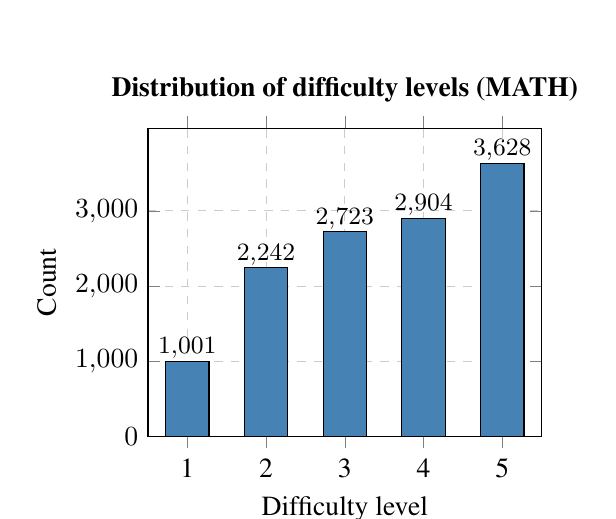
\begin{tikzpicture}
    \begin{axis}[
      ybar,
      width=0.85\linewidth,
      height=5.5cm,
      x=1cm,
      bar width=0.55cm,
      ymin=0,
      ymax=4100,
      xmin=0.5,
      xmax=5.5,
      xtick={1,2,3,4,5},
      xticklabels={1,2,3,4,5},
      ytick={0,1000,2000,3000},
      xlabel={Difficulty level},
      ylabel={Count},
      title={Distribution of difficulty levels (MATH)},
      title style={font=\bfseries},
      nodes near coords={\pgfmathprintnumber{\pgfplotspointmeta}},
      nodes near coords align={vertical},
      every node near coord/.append style={font=\small, yshift=-2.5pt},
      grid=major,
      grid style={dashed,gray!40},
    ]
    \addplot[fill=steelblue, draw=black, line width=0.4pt] coordinates {
      (1, 1001)
      (2, 2242)
      (3, 2723)
      (4, 2904)
      (5, 3628)
    };
    \end{axis}
  \end{tikzpicture}
  }
  \caption{Distribution of difficulty levels in the MATH dataset.}
  \label{fig:competition_math_difficulty}
\end{figure}

The MATH data set provides mathematical problems at the competition-level with step-by-step solutions. As shown in Figure~\ref{fig:competition_math_difficulty}, higher difficulty levels (especially level 5) account for the largest share of problems, while level 1 is relatively rare. This imbalance means the training set is dominated by challenging examples, which contributes to low baseline pass rates and makes optimization harder, particularly in early training. In contrast, GSM8K contains 7,473 grade-school math word problems that typically require fewer reasoning steps and exhibit a lower difficulty. Mixing datasets with such differing complexity levels introduces an imbalance, as over-emphasizing easier GSM8K examples may encourage superficial reasoning strategies, whereas placing too much weight on MATH early in training can destabilize optimization and hinder learning progress.

\subsection{Misalignment between Quizzes and Real Problems}
Beyond the difficulty of the data set, the misalignment of the generated quizzes also play a critical role. If intermediate quizzes are not well aligned with the according problem difficulty or reasoning requirements, the model may receive reward signals that are irrelevant to solving the original task, leading to unreal or misdirected learning. 

Conversely, if the quizzes simply restate or closely duplicate the original problem, the policy can exploit this structure by focusing only on producing the correct final answer, since success on the final answer automatically guaranties high quiz rewards. In this case, the quiz signal fails to provide additional supervision beyond the correctness of the outcome and does not encourage meaningful step-by-step reasoning.

\subsection{Complexity of Reward Engineering}
Designing reinforcement learning rewards for reasoning is inherently challenging.
The reward function must simultaneously encourage correct final answers, coherent intermediate reasoning, and well-structured solutions while remaining stable under policy optimization. 
In practice, poorly designed rewards are often vulnerable to reward hacking, where the policy maximizes reward through superficial or trivial token sequences that satisfy surface-level criteria without performing genuine reasoning. 

Prior approaches such as Math-Shepherd address this issue by training process reward models, but these models can overfit to specific linguistic or structural patterns and introduce additional optimization complexity\cite{wang2024mathshepherdverifyreinforcellms}. In contrast, our goal is to design a simple yet effective reward signal that is fully automatic and robust to exploitation under reinforcement learning.

\subsection{Hardware and Computational Constraints}
A significant and practical limitation of this work is the computational capacity. All experiments are conducted using a single NVIDIA A100 (80GB) GPU, which imposes strict constraints on model size, training strategy, and dataset scale.

Under this hardware setting, full-parameter fine-tuning of large language models is infeasible, both due to memory limitations and prohibitive training cost. As a result, all supervised fine-tuning and reinforcement learning experiments rely on Low-Rank Adaptation (LoRA)\cite{hu2021loralowrankadaptationlarge}. While LoRA significantly reduces memory usage, it also constrains the expressiveness of model updates and may limit the upper bound of achievable performance.

Similarly, it is computationally impractical to train on the full available data set with long generation lengths, large batch sizes, or extensive rollouts. Attempting to do so would lead to out-of-memory (OOM) errors or an excessive training cost. Consequently, data set filtering, reduced batch sizes, limited group sampling, and conservative rollouts configurations are necessary trade-offs.

\subsection{Thesis Objectives}

To address the challenges of scalable and reliable step-by-step reasoning in large language models,
this thesis seeks to:

\begin{enumerate}
    \item Develop a reinforcement learning training pipeline that improves mathematical reasoning
    without relying on human-annotated chains of thought, while remaining fully automated and scalable across different model sizes.

    \item Investigate the complementary roles of SFT and RL post-training for
    mathematical reasoning through controlled ablations (SFT-only, RL-only, and SFT+RL),
    evaluating whether post-training alone improves reasoning performance, and analyzing how
    its effects differ from supervised learning.

    \item Design a simplified and robust reward function that integrates step-level bonuses,
    final-answer rewards, and automatically generated quiz rewards, while remaining resistant
    to reward hacking and stable under policy optimization.

    \item Identify and reinforce weak reasoning segments by estimating chunk-level saliency from
    repeated quiz and exam feedback, selectively picking low-contribution chunks, and
    amplifying their influence during policy optimization to improve long-horizon reasoning.

    \item Evaluate the resulting models on GSM8K, MATH, MATH500, and AIME~2025, and compare their performance against SFT baselines and existing methods.
\end{enumerate}


\subsection{Expected Outcomes and Significance}

We expect the proposed framework to produce measurable improvements in mathematical benchmarks.
Beyond improvements in final-answer accuracy, the resulting models are expected to produce
solutions that exhibit more structured, coherent, and interpretable step-by-step reasoning compared to supervised fine-tuning (SFT) baselines. 
We anticipate improvements in reasoning robustness for problems that require long-horizon inference, where early errors can propagate and invalidate the final solution.

By eliminating the need for human-annotated reasoning traces, the proposed training pipeline remains
fully automated and scalable. All intermediate supervision signals are generated programmatically,
allowing the method to be applied to new domains and datasets without additional annotation cost.
This feature makes the approach suitable for large-scale or resource-constrained
research settings, where collecting high-quality process supervision is impractical.

This thesis shows that reinforcement learning can be used to shape reasoning behavior
in LLMs using simple training signals.
By emphasizing intermediate feedback and targeted reinforcement of weak reasoning segments, the
proposed approach offers a practical alternative to human-annotated process supervision, while
avoiding the limitations of outcome-only optimization.
Although this work focuses on mathematical reasoning, the underlying ideas may generalize to other
tasks that require long-horizon reasoning, such as scientific problem solving, planning, and
agent-based decision making.



\chapter{Related Work}
\section{Outcome vs. Process Supervision}
Most early approaches to mathematical reasoning in large language models rely on outcome supervision, where training optimizes only the correctness of the final answer. While simple and scalable, this paradigm provides no direct feedback on intermediate reasoning steps, allowing models to rely on shallow patterns that do not generalize well to harder problems.

The work “Let’s Verify Step by Step"\cite{lightman2023letsverifystepstep} introduces process supervision, which evaluates and rewards intermediate reasoning steps rather than only final outcomes. By training a verifier to assess step-by-step reasoning traces, the authors show that guiding the reasoning trajectory itself leads to substantial performance gains on challenging benchmarks such as MATH. This demonstrates that training objectives strongly influence reasoning behavior, and that step-level feedback can significantly improve long-horizon reasoning.

Despite its effectiveness, process supervision depends on human-annotated reasoning traces, which are costly to collect and difficult to scale across domains. Annotation quality may also introduce stylistic biases. These limitations motivate the search for automated step-level supervision mechanisms that preserve the benefits of process supervision while maintaining the scalability of outcome-based training.

\section{Pure Reinforcement Learning Approaches}
While process supervision augments outcome supervision with explicit step-level signals, an alternative line of work investigates whether reinforcement learning alone can induce reasoning behaviors without any supervised fine-tuning or annotated chains of thought. DeepSeek-R1 represents a prominent example of this direction.

DeepSeek-R1 demonstrates that large-scale reinforcement learning from outcome-based rewards can lead to the emergence of complex reasoning behaviors, including multi-step planning, self-verification, and error correction\cite{Guo_2025}. Notably, the model is trained without supervised fine-tuning on reasoning datasets or explicit process supervision. Instead, it relies on carefully designed reward signals and large-scale policy optimization to shape behavior.

One of the most striking findings of DeepSeek-R1 is that reasoning structures can emerge implicitly under sufficient optimization pressure, even when the reward is defined primarily on final outcomes. This challenges the assumption that explicit process supervision is strictly necessary for reasoning. The work highlights the power of reinforcement learning as a general-purpose mechanism for inducing structured behaviors in LLMs.

However, pure RL approaches come with important trade-offs. They typically require large-scale models, extensive compute, and massive amounts of interaction data to achieve stable and reliable reasoning. Training instability, reward hacking, and poor sample efficiency remain persistent challenges. Furthermore, the emergent reasoning behaviors are difficult to control or target, as the reward signal does not explicitly guide intermediate steps.

In contrast to DeepSeek-R1, this thesis adopts a hybrid approach: supervised fine-tuning provides a strong initialization, while reinforcement learning refines reasoning behavior through structured but automated step-level signals. Rather than relying on emergent reasoning alone, we aim to explicitly guide reasoning at the step level without resorting to human annotation or large-scale reward models.

\section{Math-Shepherd: Verify and Reinforce LLMs Step-by-Step without Human Annotations}
Math-Shepherd is one of the most closely related works to this thesis, as it proposes a framework for step-by-step reasoning supervision without human-annotated chains of thought\cite{wang2024mathshepherdverifyreinforcellms}. Instead of relying on manual annotations, Math-Shepherd combines automatic verification with Monte Carlo Tree Search (MCTS) to construct step-level training signals for reinforcement learning.

Math-Shepherd formulates reasoning as a tree-structured search problem, where each node corresponds to a partial reasoning state. Using MCTS, the method explores multiple reasoning trajectories by iteratively expanding candidate steps, evaluating them with a verifier, and propagating step-level values back through the search tree. This process produces a process-level reward signal that reflects the quality of intermediate reasoning steps rather than only final outcomes. The resulting signals are then used to reinforce the policy, enabling more precise credit assignment across reasoning steps.

A key contribution of Math-Shepherd is demonstrating that verification-guided search combined with reinforcement learning can approximate the benefits of human process supervision. By leveraging MCTS, the method explicitly reasons over alternative intermediate steps and systematically evaluates their contribution to the final answer. Empirical results show significant improvements on mathematical reasoning benchmarks, confirming that automated step-level supervision can effectively replace human-annotated reasoning traces.

However, this approach introduces substantial computational and architectural complexity. MCTS requires repeated rollouts, tree maintenance, and verifier evaluations, making training expensive and sensitive to search hyperparameters. In addition, Math-Shepherd trains a process reward model (PRM) using supervision derived from automated verification and MCTS-based search, which may still overfit to specific reasoning patterns or verification-induced biases. These factors complicate tuning and may limit scalability, especially for smaller models or resource-constrained settings.

In contrast, this thesis explores a simpler reinforcement learning framework that avoids explicit tree search and separate reward model training. Rather than performing MCTS over reasoning trajectories, we generate lightweight intermediate quizzes to probe partial reasoning states and selectively reinforce weak reasoning segments. This design preserves the core insight of Math-Shepherd, which is step-level feedback is critical for reasoning, while prioritizing simplicity, robustness, and ease of integration into standard policy optimization pipelines.

% \section{Reinforcement Learning for Reasoning in Small LLMs: What Works and What Doesn’t}
% Recent work on reinforcement learning for reasoning has largely focused on large-scale models, often obscuring the practical limitations faced by smaller LLMs. The study “Reinforcement Learning for Reasoning in Small LLMs: What Works and What Doesn’t” systematically investigates which reinforcement learning techniques are effective under tight compute and data constraints.

% This work evaluates a range of RL strategies on relatively small models, demonstrating that many techniques successful at scale fail to transfer directly. In particular, complex reward models, dense supervision, and aggressive optimization often lead to instability or negligible gains. Instead, the authors find that simple reward designs, careful curriculum selection, and selective reinforcement are critical for improving reasoning performance in smaller models.

% This study showed us that reward simplicity and alignment matter more than expressiveness when resources are limited. Overly complex reward functions increase the risk of reward hacking and optimization instability, while simpler rewards and properly aligned can still produce meaningful reasoning improvements.

% This finding strongly aligns with the design philosophy of this thesis. By using lightweight step bonuses, final-answer rewards, and automatically generated quiz rewards, we prioritize robustness and scalability over reward model complexity. Additionally, our strategy of cherry-picking weak reasoning chunks echoes the study’s emphasis on targeted reinforcement as a practical mechanism for improving reasoning under constrained settings.

\section{R1-Searcher: Incentivizing the Search Capability in LLMs via Reinforcement Learning}
R1-Searcher investigates how reinforcement learning can be used to explicitly incentivize search behaviors in large language model\cite{song2025r1searcherincentivizingsearchcapability}. Rather than focusing solely on final answer correctness, the work emphasizes the importance of intermediate exploration steps, showing that structured search policies can emerge when models are rewarded for effective information gathering and reasoning progression.

This work is closely related to our thesis in its recognition that reasoning is a sequential decision-making process, where intermediate actions critically influence final outcomes. However, R1-Searcher primarily targets retrieval and search efficiency, whereas our work focuses on improving internal reasoning quality through quiz-based intermediate evaluation. Both approaches highlight the importance of shaping intermediate behaviors via reinforcement learning rather than relying on outcome-only rewards.

\section{Agent Lightning: Training General-Purpose Agents with Reinforcement Learning}
Agent Lightning presents a general framework for training AI agents using reinforcement learning under a Partially Observable Markov Decision Process (POMDP) formulation\cite{luo2025agentlightningtrainai}. The work emphasizes modular reward design, long-horizon optimization, and scalability across tasks.

This perspective directly informs the theoretical framing of our work. By treating reasoning as a sequential decision process with partial observability, Agent Lightning provides a conceptual foundation for our quiz–exam reward structure and chunk-level saliency analysis. Our work can be viewed as a specialization of this agent-centric view, where the environment is a reasoning task and rewards are derived from intermediate quizzes and final answer evaluation.

\section{Datasets and Data Augmentation}
\subsection{Overview of MATH and GSM8K}
MATH and GSM8K are two widely used benchmarks for evaluating mathematical reasoning in large language models, representing distinct difficulty regimes. The MATH dataset contains competition-level problems that require long-horizon, multi-step reasoning and precise symbolic manipulation, resulting in low baseline pass rates and making it a challenging test of deep reasoning ability\cite{hendrycksmath2021}. In contrast, GSM8K consists of grade-school word problems that typically require fewer reasoning steps and exhibit lower intrinsic difficulty, while still demanding accurate numerical reasoning and language understanding\cite{cobbe2021trainingverifierssolvemath}.

Prior work has observed that mixing these datasets during training introduces curriculum trade-offs. Over-emphasizing GSM8K may encourage shallow or pattern-based strategies, whereas prioritizing MATH too early can hinder optimization and destabilize learning. These challenges motivate training strategies that can adapt to varying difficulty levels and provide guidance beyond final-answer supervision.

\subsection{MetaMathQA Synthetic Dataset}
MetaMathQA is a large-scale synthetic dataset constructed from the training splits of MATH and GSM8K, designed to improve supervised initialization for mathematical reasoning\cite{yu2024metamathbootstrapmathematicalquestions}. By generating diverse solution formats and reasoning traces using language models, MetaMathQA expands data coverage without leaking test examples. Supervised fine-tuning on MetaMathQA has been shown to significantly improve downstream reasoning performance and stabilize subsequent reinforcement learning.

However, MetaMathQA primarily provides outcome-level supervision and does not guarantee the correctness or usefulness of intermediate reasoning steps. As a result, models fine-tuned on MetaMathQA may still rely on surface-level reasoning patterns. In this thesis, MetaMathQA is used as a strong initialization, while reinforcement learning with automated step-level signals is employed to further refine reasoning behavior and address the limitations of synthetic supervision.

\subsection{Summary}

Prior work highlights a broad spectrum of approaches to training reasoning-capable large language
models, ranging from outcome-only supervision to human-annotated process supervision and pure
reinforcement learning. A common conclusion across these lines of work is that effective reasoning
requires guidance beyond final-answer correctness alone. Methods that incorporate step-level
feedback—whether through human annotations, automated verification, or search-based evaluation—
consistently demonstrate stronger performance on long-horizon reasoning tasks.

At the same time, existing approaches expose important trade-offs. Human-annotated process
supervision offers strong empirical gains but suffers from limited scalability and high annotation
costs. Pure reinforcement learning can induce emergent reasoning behaviors, yet typically demands
substantial computational resources and large-scale optimization. Hybrid methods such as
Math-Shepherd bridge part of this gap by introducing automated, verification-based rewards, but
at the cost of significantly increased training and inference complexity due to MCTS-based reasoning
exploration.

Building on these insights, this thesis positions itself within the design space between expressive but
expensive process supervision and scalable but sparse outcome-only optimization. Rather than
relying on human annotations, heavy reward models, or large-scale search, we explore whether
simple, automated, and hardware-feasible reinforcement learning signals can approximate the
benefits of process supervision. By focusing on step-level credit assignment, selective reinforcement
of weak reasoning segments, and robust reward design, this work aims to provide a practical and
scalable path toward improving long-horizon reasoning in large language models. The proposed
approach and its empirical evaluation are detailed in the following methodology, experiments, and
results.


\chapter{Methodology}
This section presents the training pipeline used to improve step-by-step mathematical reasoning in large language models. We first apply Low-Rank Adaptation (LoRA) with supervised fine-tuning on a synthetic mathematics dataset (MetaMathQA) to obtain a strong initialization. After merging the LoRA parameters into the base model, reinforcement learning is applied to further refine reasoning behavior using automatically computed rewards. The proposed methodology emphasizes sequence-level optimization, scalable reward design, and targeted reinforcement of reasoning quality without relying on human-annotated intermediate steps.

\section{Parameter-Efficient Adaptation with LoRA}
To efficiently adapt large language models for mathematical reasoning, we employ Low-Rank Adaptation (LoRA) during the supervised fine-tuning stage. LoRA injects trainable low-rank matrices into selected linear layers while keeping the base model parameters frozen, significantly reducing memory usage and training cost.

We apply LoRA to both attention and feed-forward submodules, including:
\[
\{ \texttt{q\_proj}, \texttt{k\_proj}, \texttt{v\_proj}, \texttt{o\_proj},
   \texttt{gate\_proj}, \texttt{up\_proj}, \texttt{down\_proj} \}.
\]

Each adapted weight matrix $W$ is reparameterized as:
\begin{align}
W' &= W + \Delta W, \\
\Delta W &= AB,
\end{align}

where $A \in \mathbb{R}^{d \times r}$ and $B \in \mathbb{R}^{r \times k}$ and rank $r$ denotes the low-rank dimension of the adaptation. In our experiments, we set the LoRA rank to $r=16$, the scaling factor to $\alpha=64$, and the dropout probability to $0.05$. This design allows the model to acquire task-specific reasoning behaviors during supervised fine-tuning while preserving the general knowledge encoded in the pretrained backbone.

\section{Model Initialization and Supervised Fine-Tuning}
We initialize our models Qwen2.5-7B\cite{qwen2025qwen25technicalreport} using supervised fine-tuning on MetaMathQA, a synthetic dataset containing step-by-step mathematical solutions.

During SFT, only LoRA parameters are optimized, while the base model remains frozen. Training minimizes the standard cross-entropy loss over the entire generated sequence, encouraging the model to produce structured reasoning steps followed by a concise final answer.

To improve training stability and hardware efficiency, we employ dynamic sequence padding with padding aligned to multiples of 8 and mask padded tokens using a label value of $-100$. We use a per-device batch size of 8 with gradient accumulation over 8 steps, resulting in an effective batch size of 64. The learning rate is set to $1 \times 10^{-4}$ with a warmup ratio of 0.05, and training is conducted for 3 epochs. All experiments are performed in \texttt{bfloat16} precision with gradient norm clipping at 1.0 to prevent instability.

After SFT converges, the LoRA adapters are merged into the base model weights, yielding a single consolidated checkpoint. This merged model is then used as the initialization policy for subsequent reinforcement learning with GRPO\cite{shao2024deepseekmathpushinglimitsmathematical}.

\section{Reinforcement Learning Algorithm}
After merging LoRA weights into the base model, we apply reinforcement learning using Group Relative Policy Optimization (GRPO). At this stage, all model parameters are trainable, and optimization is performed via full-parameter tuning. Given a question $q$, GRPO samples a group of $G$ complete outputs:
\begin{align}
o_1, o_2, \ldots, o_G 
&\sim \pi_{\theta_{\text{old}}}(\cdot \mid q).
\end{align}

Each output receives a scalar reward $r_i = R(q, o_i)$. 
Instead of training a value function, GRPO computes group-relative advantages:
\begin{align}
A_i 
&= \frac{r_i - \operatorname{mean}(r_1, \ldots, r_G)}
        {\operatorname{std}(r_1, \ldots, r_G)}.
\end{align}

The policy is optimized by maximizing:
\begin{align}
J_{\text{GRPO}}(\theta)
&= \mathbb{E}\!\left[
q \sim P(Q),\;
\{o_i\}_{i=1}^{G} \sim \pi_{\theta_{\text{old}}}(\cdot \mid q)
\right] \nonumber \\
&\quad \left[
\frac{1}{G} \sum_{i=1}^{G}
\min\Big(
\rho_i(\theta) A_i,\;
\operatorname{clip}\big(\rho_i(\theta), 1-\epsilon, 1+\epsilon\big) A_i
\Big)
\right]
- \beta\, D_{\mathrm{KL}}\!\left(
\pi_\theta \,\|\, \pi_{\text{ref}}
\right).
\end{align}

where 
\begin{align}
\rho_i(\theta) = 
\frac{\pi_\theta(o_i \mid q)}
     {\pi_{\theta_{\text{old}}}(o_i \mid q)}
\end{align}     
is the importance sampling ratio, 
$\epsilon$ is the clipping threshold, 
and $\beta$ controls the strength of the KL regularization. This formulation encourages the model to prefer reasoning trajectories that perform better relative to alternatives generated for the same question.

\section{Reward Modeling}
\label{sec:reward-modeling}
To provide informative training signals for long-horizon reasoning without human-annotated traces,
we design an reward function that decomposes feedback into three components:
a step bonus, a final-answer exam reward, and  intermediate quiz rewards.
Figure~\ref{fig:reward_structure} summarizes the overall computation flow.

\begin{figure}[H]
    \centering
    \includegraphics[width=0.89\textwidth, trim=0 120 0 100, clip]{Image/RewardStructure.jpg}
    \caption{Overview of the proposed automatic reward design.
The total reward combines step bonus, exam reward, and a clipped quiz reward computed from intermediate quizzes on partial reasoning chunks.}
    \label{fig:reward_structure}
\end{figure}

The total reward for an output $o$ is defined as:
\begin{equation}
R(q,o) = R_{\text{step}} + R_{\text{exam}} + R_{\text{quiz}}
\end{equation}

The quiz reward is computed as the average score over all generated quizzes:
\begin{equation}
R_{\text{quiz}} = \lambda_{\text{quiz}} \cdot \frac{1}{N_q}
\sum_{j=1}^{N_q} E_j ,
\end{equation}

where $N_q$ denotes the number of quizzes generated from the reasoning trace, and $E_j \in [0,1]$
indicates whether the $j$-th quiz is answered correctly.


\begin{enumerate}
    \item \textbf{Step bonus} encourages explicit and structured reasoning by rewarding the
    presence of a sufficient number of reasoning steps in the generated solution.

    \item \textbf{Exam reward} evaluates final-answer correctness by comparing the predicted
    answer against the ground truth using exact match (EM) and token-level F1 metrics.

    \item \textbf{Quiz reward} assesses intermediate reasoning quality by answering automatically
    generated quizzes conditioned on partial reasoning chunks.
\end{enumerate}

All reward components are computed after the full reasoning trace is generated, ensuring that
intermediate supervision is applied at the sequence level while maintaining a simple and stable
optimization objective.


\subsection{Step Bonus}
To discourage premature guessing and encourage explicit reasoning, we include a simple step-based bonus. Let $n_{\text{steps}}$ denote the number of extracted reasoning steps and $n_{\min}$ the minimum required number of steps. Given a maximum bonus $b$, the step reward is defined as:
\begin{equation}
r_{\text{step}} =
\begin{cases}
b, 
& n_{\text{steps}} \ge n_{\min} 
\quad \text{(binary mode)}, \\[6pt]

b \cdot \min\!\left(1, \dfrac{n_{\text{steps}}}{n_{\min}}\right), 
& \text{(ratio mode)}, \\[6pt]

0, 
& \text{otherwise}.
\end{cases}
\end{equation}

\subsection{ Exam Reward}
The exam reward focuses on the correctness of the final answer and serves as the
dominant training signal. Let $p$ denote the predicted final answer and $G$ the
set of ground-truth answers. We compute the token-level F1 score
$F1(p, G) \in [0,1]$.

Instead of using a binary decision rule, we adopt a clipped, normalized reward
based on the F1 score, controlled by a threshold parameter $\tau_{\text{exam}}$:

\begin{equation}
r_{\text{exam}}
= \max\!\left(
0,\;
\min\!\left(
1,\;
\frac{F1(p, G)}{\tau_{\text{exam}}}
\right)
\right).
\end{equation}

This formulation provides partial credit for partially correct answers while preventing excessively large rewards through clipping.

When operating in exact-match-only mode, we prioritize strict answer correctness
by assigning a full reward to exact matches, while still providing limited
partial credit based on token-level overlap.

\begin{equation}
r_{\text{exam}} =
\begin{cases}
1.0, 
& EM(p, G) \ge 1.0, \\[6pt]
0.5 \cdot F1(p, G), 
& \text{otherwise}.
\end{cases}
\end{equation}


If the model fails to produce a valid final answer, we directly set
$r_{\text{exam}} = -1$. This formulation enforces a sharp decision boundary and
avoids ambiguous partial credit.

\subsection{Quiz Reward}
\label{sec:quiz-reward}
To provide intermediate supervision without human annotations, we generate a set of short quiz questions targeting intermediate reasoning states. Each quiz is answered using a corresponding reasoning chunk, and its answer is evaluated against a gold answer.

For quiz $j \in \{1, \ldots, N_Q\}$, let the quiz-level reward be
\begin{equation}
E_j =
\begin{cases}
+1, & F1_j \ge \tau_{\text{quiz}}, \\[6pt]
0, & \text{otherwise}.
\end{cases}
\end{equation}

The total quiz reward is defined as
\begin{equation}
r_{\text{quiz}}
= \lambda_{\text{quiz}} \cdot
\frac{1}{N_Q} \sum_{j=1}^{N_Q} E_j,
\end{equation}

where $\lambda_{\text{quiz}}$ controls the overall weight of the quiz reward and
$c$ prevents extreme gradients when many quizzes are answered correctly or
incorrectly. If no quizzes are defined for a problem, we set $r_{\text{quiz}} = 0$. This quiz-based reward provides dense intermediate feedback while remaining fully automated, enabling step-level supervision without requiring any human-annotated reasoning traces.

\section{Training Template}
\label{sec:training-templates}
To ensure consistent and parseable reasoning behavior, we define fixed prompt templates for all stages of the pipeline. The exact templates are provided in Appendix \ref{app:prompt}–~\ref{app:quiz-question-alignment}.

\paragraph{Solution generation (Appendix~\ref{app:prompt}).}
The model is instructed to produce explicit reasoning steps (e.g., ``Step~1'', ``Step~2'', \ldots) followed by a single final answer in a strict \texttt{<final\_answer>} tag. This structure enables reliable extraction of both step boundaries for chunk-level evaluation and final answers scoring.

\paragraph{Quiz answering (Appendix~\ref{app:quiz-prompt}).}
Given an original question, a partial reasoning chunk, and a quiz, the model outputs only a short answer token (e.g., a number or letter) with no additional reasoning. This ensures answers are grounded in the provided chunk and directly comparable to gold answers.

\paragraph{Quiz generation (Appendix~\ref{app:quiz-generation-prompt}).}
Quizzes are generated based on the original problem and its correct solution. The prompt requires that quizzes target numerical or symbolic checkpoints, produce short unambiguous answers, and output in JSON format for automatic parsing.

\paragraph{Quiz--question alignment verification (Appendix~\ref{app:quiz-question-alignment}).}
A separate model judges whether each generated quiz is appropriately aligned with the original problem. Quizzes that are misaligned or that merely restate the final goal are filtered out, preventing the model from exploiting trivial reward shortcuts.

\section{Saliency over Reasoning Chunks}
\label{sec:saliency_over_chunk}
Repeat the \emph{same} adversarial quizzes and the user exam $K$ times. Let $Q_{k,j}$ be the normalized quiz reward for chunk $j$ on run $k$, and $E_k$ the exam reward on run $k$. Define

\medskip
\noindent\textbf{Exam-weighted chunk saliency:}
\begin{equation}\label{eq:exam-weighted-saliency-formula}
s_j=\frac{1}{K}\sum_{k=1}^{K} Q_{k,j}\,E_k,\qquad
\end{equation}

\noindent\textbf{Clip positive map + normalize to a distribution:}
\begin{equation}
\tilde{s}_j=\max(0,s_j),\qquad
w_j=\frac{\tilde{s}_j}{\sum_{i=1}^{J}\tilde{s}_i},
\end{equation}
where $w_j\in[0,1]$ and $\sum_j w_j=1$. (For step-level saliency, distribute $w_j$ evenly across steps in chunk $j$.)

\paragraph{Example (Saliency Map).}
We repeat the same exam $K=3$ times with fixed quizzes and ground truths.
There are $J=3$ reasoning chunks. Each run produces quiz rewards $Q_{k,j}$
and an exam reward $E_k$. Suppose
\begin{equation}
Q_{k,j} =
\begin{bmatrix}
+0.6 & +0.2 & +0.9\\
+0.5 & 0.0 & +0.8\\
0.0 & 0.0 & +0.4
\end{bmatrix},
\qquad
E = [ +1.0,\ +0.9,\ 0.5 ].
\end{equation}
Each row corresponds to a run ($k=1,2,3$) and each column to a chunk ($j=1,2,3$).

\noindent\textbf{Step 1: Compute exam-weighted chunk saliency.}
\begin{equation}
s_j=\frac{1}{K}\sum_{k=1}^{K} Q_{k,j}E_k.
\end{equation}
Hence,
\begin{align}
s_1 &= \frac{1}{3}\bigl(0.6\times1.0 + 0.5\times0.9 + (0.0)\times(0.5)\bigr)=0.35,\\
s_2 &= \frac{1}{3}\bigl(0.2\times1.0 + (0.0)\times0.9 + (0.0)\times(0.5)\bigr)=0.07,\\
s_3 &= \frac{1}{3}\bigl(0.9\times1.0 + 0.8\times0.9 + 0.4\times(0.5)\bigr)=0.6.
\end{align}

\noindent\textbf{Step 2: Clip negatives and normalize.}
\begin{equation}
\tilde{s}_j=\max(0,s_j),\qquad
w_j=\frac{\tilde{s}_j}{\sum_{i=1}^{J}\tilde{s}_i}.
\end{equation}
Thus,
\begin{equation}
\tilde{s} = [0.35,\ 0.07,\ 0.6],\qquad
w = [0.34,\ 0.06,\ 0.58].
\end{equation}

\noindent\textbf{Interpretation.}
Chunk 3 contributes $\approx 60\%$ of the exam success, chunk 1 contributes $\approx 34\%$,
and chunk 2 only $\approx 6\%$, indicating that chunk 2 is the weakest part of the reasoning trace.


\section{Saliency-Guided Reward Reweighting in GRPO}
\label{sec:targeting-weak-chunk}

Given the chunk-level saliency distribution $\{w_j\}_{j=1}^{J}$ defined in Section~\ref{sec:saliency_over_chunk}, we identify reasoning chunks that contribute little to final exam success and selectively reinforce the corresponding training problems with GRPO.

The key idea is to operate entirely at the \emph{reward level}
rather than modifying the GRPO advantage formula or its clipped objective, 
we adjust the scalar reward returned to the trainer so that problems containing weak reasoning patterns 
receive amplified reward deviations within each group. This design keeps the approach compatible with any 
standard GRPO implementation (e.g., the TRL library's \texttt{GRPOTrainer}) without requiring changes to 
the optimization loop itself.

\subsubsection{Building the Weak-Chunk Database}
\label{sec:weak-chunk-db}

The saliency analysis described in Section~\ref{sec:saliency_over_chunk} produces, for every analyzed problem, a normalized weight vector $\mathbf{w} = (w_1, \dots, w_J)$ over its $J$ reasoning chunks.  We say a problem \emph{contains a weak chunk} if at least one of its chunks falls below a saliency threshold $\delta$:
%
\begin{equation}
  \mathcal{W}_q \;=\; \bigl\{\, j \;\bigm|\; w_j \le \delta \,\bigr\},
  \label{eq:weak-set}
\end{equation}
%
where $\delta = 0.10$ in our experiments.  For each such problem $q$, we store a pre-computed \emph{weak-chunk intensity} score
%
\begin{equation}
  \bar{m}_q \;=\; \frac{|\mathcal{W}_q|}{J},
  \label{eq:m-bar}
\end{equation}
%
which represents the fraction of reasoning chunks classified as weak.  These entries are turned into a static lookup table (the weak-chunk database), keyed by the problem identifier.
The database is constructed offline and remains fixed throughout GRPO training.  This static design avoids the computational cost of re-running saliency analysis during training.



\subsubsection{Reward-Level Weak-Chunk Focusing}
\label{sec:reward-focusing}

During GRPO training, the trainer samples a group of $G$ complete reasoning trajectories 
\[
\{o_1, \dots, o_G\}
\sim
\pi_{\theta_{\mathrm{old}}}(\cdot \mid q),
\] for each question $q$.  
Each trajectory receives a scalar reward $r_i = R(q, o_i)$ computed from the three 
reward components (step bonus, exam reward, and quiz reward) defined in Section~\ref{sec:reward-modeling}.

For questions that appear in the weak-chunk database, we apply a \emph{reward-level focusing} adjustment that 
amplifies each trajectory's deviation from the group mean:
%
\begin{equation}
  r'_i \;=\; r_i \;+\; \kappa \cdot \bar{m}_q \cdot \bigl(r_i - \mu_{\mathrm{group}}\bigr),
  \label{eq:reward-focus}
\end{equation}
%
where $\mu_{\mathrm{group}} = \frac{1}{G}\sum_{i=1}^{G} r_i$ is the mean reward within the group, $\bar{m}_q$ is the pre-computed weak-chunk intensity from Equation~\eqref{eq:m-bar}, and $\kappa > 0$ is a focus coefficient.  For problems not in the weak-chunk database, $\bar{m}_q = 0$ and the reward remains unchanged.

The effect of Equation~\eqref{eq:reward-focus} is intuitive. In a group of trajectories for a weak-chunk problem, trajectories that score above the group mean have their reward increased, while those scoring below the mean have their reward decreased.  The magnitude of this shift is proportional to both the focus coefficient $\kappa$ and the fraction of weak chunks $\bar{m}_q$. This amplification increases the selection pressure within weak-chunk problems, 
encouraging the policy to move away from lower reward reasoning trajectories 
and toward higher reward alternatives. 
If the reward gap is primarily driven by weak reasoning segments, 
this mechanism indirectly promotes trajectories that repair those segments 
in subsequent rollouts.


\paragraph{Relationship to advantage scaling.}

An alternative approach would directly scale the GRPO advantage,
such as $\hat{A}_i = (1 + \kappa \bar{m}_q) A_i$.
However, this is not mathematically equivalent to the reward-level
formulation in Equation~\eqref{eq:reward-focus}.
Direct advantage scaling modifies the gradient magnitude after
normalization, whereas reward-level focusing reshapes the reward
distribution itself and therefore alters both the group variance
and the subsequent normalization step.
As a result, the two methods may lead to different optimization
dynamics in practice.



% \subsection{Identifying weak chunks.}
% Let $\mathcal{W} \subseteq \{1,\dots,J\}$ denote the set of low-saliency chunks:
% \begin{equation}
% \mathcal{W} =
% \begin{cases}
% \arg\operatorname{bottom}_k \{ w_j \}, & \text{(lowest-$k$ chunks)}, \\
% \{ j \mid w_j \le \delta \}, & \text{(below threshold $\delta$)}.
% \end{cases}
% \end{equation}

% \subsection{GRPO group advantages.}
% For a given question $q$, GRPO samples a group of $G$ complete reasoning trajectories
% $\{o_1,\dots,o_G\} \sim \pi_{\theta_{\text{old}}}(\cdot \mid q)$.
% Each trajectory receives a scalar reward $r_i$, and the standard GRPO advantage is computed as
% \begin{equation}
% A_i =
% \frac{
% r_i - \operatorname{mean}(\{r_1,\dots,r_G\})
% }{
% \operatorname{std}(\{r_1,\dots,r_G\})
% }.
% \end{equation}

% \subsection{Weak-chunk-aware advantage scaling.}
% To emphasize trajectories that expose weak reasoning segments, we define a weak-chunk indicator:
% \begin{equation}
% m_j = \mathbb{1}\{ j \in \mathcal{W} \},
% \end{equation}

% and aggregate it at the trajectory level as
% \begin{equation}
% \bar m_i = \frac{1}{J} \sum_{j=1}^{J} m_{i,j}.
% \end{equation}

% We then define an adjusted advantage as
% \begin{equation}
% \hat A_i = (1 + \kappa \bar m_i) A_i,
% \end{equation}
% where $\kappa > 0$ is a focus coefficient. Trajectories that contain weak reasoning chunks therefore receive amplified gradient magnitudes, enabling targeted credit assignment.

% \subsection{GRPO objective with weak-chunk focus.}
% Let the importance ratio be
% \begin{equation}
% \rho_i(\theta) =
% \frac{\pi_\theta(o_i \mid q)}{\pi_{\theta_{\text{old}}}(o_i \mid q)}.
% \end{equation}
% The weak-chunk-aware GRPO objective is
% \begin{equation}
% \mathcal{L}_{\text{GRPO}}^{\text{focus}}
% =
% \mathbb{E}
% \left[
% \frac{1}{G}
% \sum_{i=1}^{G}
% \min
% \left(
% \rho_i(\theta)\hat A_i,
% \operatorname{clip}(\rho_i(\theta), 1-\epsilon, 1+\epsilon)\hat A_i
% \right)
% \right]
% -
% \beta D_{\mathrm{KL}}(\pi_\theta \,\|\, \pi_{\text{ref}}).
% \end{equation}

% \paragraph{Stopping criterion.}
% The stopping criterion operates at the level of chunk saliency estimation and is therefore independent of the GRPO. A chunk $j \in \mathcal{W}$ is removed from the weak set once its estimated contribution improves:
% \begin{equation}
% \Delta w_j = w^{\text{new}}_j - w^{\text{old}}_j \ge \eta
% \quad \text{or} \quad
% \Delta Q_j \ge \eta,
% \end{equation}
% where $Q_j$ denotes the normalized quiz reward associated with chunk $j$.

% \paragraph{Example.}
% Assume $T=6$ reasoning steps with chunk size $m=2$, resulting in $J=3$ chunks.
% The estimated saliency distribution is
% \[
% w = [0.22,\; 0.53,\; 0.00],
% \]
% so the weakest chunk is $\mathcal{W}=\{3\}$.

% For a GRPO group of $G=4$ trajectories, suppose the normalized group-relative advantages are
% \[
% A = [0.40,\; 0.30,\; 0.10,\; -0.10],
% \]
% and the weak-chunk indicators are
% \[
% \bar m = [0,\; 0,\; 1,\; 1].
% \]
% With $\kappa = 1.0$, the adjusted advantages become
% \[
% \hat A = [0.40,\; 0.30,\; 0.20,\; -0.20].
% \]

% Thus, trajectories that contain weak reasoning chunks receive stronger positive or negative gradients, accelerating improvement on deficient reasoning segments while preserving GRPO’s group-relative and clipped optimization structure.


\chapter{Experiments and Results}

This chapter presents the experimental setup and evaluation methodology used to assess the effectiveness of the proposed step-level reinforcement learning framework. We describe the datasets preprocessing, model configurations, training procedure, and evaluation metrics, followed by an analysis of experimental outcomes. Where final numerical results are not yet fixed, we report observations that are directly supported by logged training runs and clearly indicate where results remain under consolidation.

\section{Experimental Setup}

\subsection{Data Preparation and Quiz Quality Filtering}

Reinforcement learning is conducted on a combined training set consisting of GSM8K and MATH, with a total of 14,973 examples. For each problem, GPT-5-mini is used to  generate a small set of intermediate quizzes derived from the original question, with the number of quizzes varying between one and three. To ensure that these quizzes meaningfully target potential reasoning errors rather than superficial cues, we employ GPT-5.2 to implement a three-level quality classification framework. This framework evaluates the alignment between the generated adversarial quizzes and the corresponding original math problems, filtering out low-quality cases.

\begin{enumerate}
  \item \textbf{Good.}
  Quizzes that are both grounded in the problem context and useful for
  verifying intermediate reasoning steps. These quizzes target critical
  checkpoints in the solution process, such as intermediate calculations,
  unit conversions, or partial results.

  \item \textbf{\flag{ok\_final}.}
  Quizzes that, while grounded and potentially useful, sometimes restate
  the original question's final goal or ask for the same final quantity.
  These quizzes do not effectively probe intermediate reasoning skills and are thus classified separately from high-quality adversarial quizzes.

  \item \textbf{Bad.}
  Quizzes that fail to meet alignment criteria, either not grounded in the
  problem's context, not useful for checking reasoning steps, or both.
  These include quizzes that ask about irrelevant information, contain
  logical inconsistencies, or cannot be answered using information from
  the original problem.
\end{enumerate}

\begin{figure}[tbp]
  \centering
  \includegraphics[height=0.45\textheight,keepaspectratio]{Image/QuizGeneratePipeline.png}
  \caption{Quiz generation and quality filtering pipeline.}
  \label{fig:quiz-generate-pipeline}
\end{figure}

Then, the verifier model (GPT-5.2) assigns an \code{overall\_ok} flag to each problem--quiz pair set. This flag is set to False if any quiz in the set is labeled as bad, ensuring strict quality control. We observed that
approximately 791 problems ($\sim$5.3\% of the dataset) consistently produced only bad quizzes on multiple generation attempts. These problems were
often too simple or straightforward, lacking sufficient intermediate steps to generate meaningful adversarial quizzes.

We removed 791 problematic instances from the original merged data set, retaining only samples with \code{overall\_ok = True}. This filtering step
ensures that the model is trained exclusively on high-quality, well-aligned adversarial quizzes that genuinely probe intermediate mathematical reasoning
rather than trivially restating the final question. After quality filtering, the final training set contains 14{,}183 math problems paired with 41{,}376
adversarial quizzes, averaging approximately 2.9 quizzes per problem. The resulting training corpus therefore consists of 55{,}559 instances (14{,}183
original problems and 41{,}376 quiz--answer pairs), forming a clean and well-aligned dataset for reinforcement learning.

\subsection{Baseline Model Configuration}
\label{sec:baseline_model_config}
To evaluate the effectiveness of step-level reinforcement learning across different model scales, we consider two baseline language models: Qwen2.5-7B-Instruct and Qwen2.5-3B-Instruct. These models belong to the same architecture family and share an identical decoder-only Transformer structure, differing only in parameter count. This design allows us to isolate the effect of model capacity when analyzing reinforcement learning signals.

All baseline models are first initialized through supervised fine-tuning (SFT) on the MetaMathQA dataset using Low-Rank Adaptation (LoRA). During this stage, the base model parameters remain frozen, and only the LoRA parameters are optimized. This parameter-efficient setup reduces memory overhead and improves training stability while enabling the model to acquire task-specific mathematical reasoning behaviors.

After supervised fine-tuning converges, the trained LoRA adapters are merged into the base model weights, producing a single consolidated checkpoint for each model size. The resulting merged models serve as SFT baselines and represent the final output of the supervised learning stage.

For reinforcement learning post-training, we attach a new set of LoRA adapters to these merged SFT models and apply Group Relative Policy Optimization (GRPO). This separation ensures that the reinforcement learning phase is built upon a fixed SFT-initialized policy, while allowing reinforcement learning updates to be applied independently through newly introduced low-rank parameters.

Baseline performance is evaluated after supervised fine-tuning and prior to any reinforcement learning updates. This evaluation provides a clean reference point that allows us to attribute subsequent performance changes specifically to the effects of reinforcement learning.

\subsection{Reinforcement Learning Procedure}
\label{sec:rl-procedure}

Following supervised initialization, we further optimize the policy using
Group Relative Policy Optimization (GRPO), a method that avoids
training a value function by computing \emph{group-relative}
advantages from multiple sampled completions per prompt.

\paragraph{Initialization and parameterization.}
We start from the SFT pretrained checkpoint and load it as the initial policy.
In our implementation, the policy is instantiated through an \texttt{ExamModel}
wrapper that (i) ensures a valid \texttt{pad\_token} by falling back to the
\texttt{eos\_token} when needed, and (ii) applies parameter-efficient adaptation via LoRA on both attention and MLP projection layers as shown below:
\[
\{ \texttt{q\_proj}, \texttt{k\_proj}, \texttt{v\_proj}, \texttt{o\_proj},
   \texttt{gate\_proj}, \texttt{up\_proj}, \texttt{down\_proj} \}.
\]

with rank \(r=128\), scaling \(\alpha=256\), and dropout \(0.05\).
To improve memory efficiency for long generations, we enable gradient
checkpointing and disable KV-cache during training (i.e., \texttt{use\_cache=False}).

\paragraph{Training data and prompt format.}
GRPO is trained on a mixed dataset of GSM8K and MATH training problems with pre-generated intermediate quizzes and gold answers. Each training example contains the original question $q$, the ground-truth final answer, and a small set of quizzes,
\[
\{(q_j^{\text{quiz}}, a_j^{\text{quiz}})\}_{j=1}^{N_q},
\quad N_q \in \{1,2,3\}.
\]
, where \(N_q\) varies between 1 and 3.
At training time, each question is formatted into a fixed template that enforces:
(1) explicitly separated reasoning steps (e.g., \texttt{Step 1:}, \texttt{Step 2:}, \dots), and (2) a single final answer in a strict XML-like tag \texttt{<final\_answer>...</final\_answer>}.
The exact prompt templates are provided in the Appendix~\ref{app:prompt} and related appendix sections.

\paragraph{Generation and group sampling.}
For each input question \(q\), GRPO samples a group of \(G\) candidate outputs:
\[
o_1, o_2, \dots, o_G \sim \pi_{\theta_{\text{old}}}(\cdot \mid q),
\]
where \(\pi_{\theta_{\text{old}}}\) denotes the policy before the current update.
In our runs, we use \(G=3\) generations per prompt.
To keep rollouts efficient, we enable vLLM-based decoding in \texttt{colocate}
mode (single-GPU setting) with \texttt{vllm\_gpu\_memory\_utilization=0.45}.
Sampling uses \(\texttt{temperature}=0.6\), \(\texttt{top\_p}=0.95\),
and \(\texttt{max\_tokens}=256\), and generation is terminated early when
encountering \texttt{</final\_answer>} or the EOS token.

\paragraph{Reward computation.}
Each sampled output \(o_i\) receives a scalar reward \(r_i = R(q,o_i)\).
In our framework, the total reward combines three components:
(i) a step structure bonus, (ii) an exam reward for final answer correctness, and (iii) a quiz reward that evaluates intermediate reasoning via quizzes:
\[
R(q,o) \;=\; R_{\text{step}}(o)\;+\;R_{\text{exam}}(q,o)\;+\;\lambda_{\text{quiz}}\,
\cdot\frac{1}{N_Q} \sum_{j=1}^{N_Q} R^{j}_{\text{quiz}},.
\]

We parses the model output by extracting
\texttt{Step k: ...} blocks and the content inside
\texttt{<final\_answer>...</final\_answer>}. Outputs that fail formatting (e.g., missing final tag) receive a negative  reward $-1$.

\emph{Exam reward.}
Let \(\mathrm{F1}(p,G)\in[0,1]\) denote the token level F1 between the predicted final
answer \(p\) and the gold set \(G\). We use a normalized, bounded exam score:
\[
R_{\text{exam}}(q,o)
=\max\!\Big(0,\; \min\!\big(1,\; \mathrm{F1}(p,G) / \tau_{\text{exam}}\big)\Big),
\]
where \(\tau_{\text{exam}}=0.6\) controls how quickly partial credit saturates.

\emph{Step bonus.}
To discourage premature guessing and encourage explicit reasoning structure,
we include a step-based bonus computed from the number of extracted steps
\(n_{\text{steps}}\). Let \(n_{\min}=1\) be the minimum required number of steps
and \(b=0.5\) the maximum bonus. We use a binary mode in below formulation:
\[
R_{\text{step}}(o)=
\begin{cases}
b, & n_{\text{steps}}\ge n_{\min} \quad(\text{binary mode}),\\
b\cdot \min\!\left(1,\frac{n_{\text{steps}}}{n_{\min}}\right),
& (\text{ratio mode}),\\
0, & \text{otherwise}.
\end{cases}
\]
This reward is only a small shaping term and is not intended to replace final
answer supervision.

\emph{Quiz reward.}
For each problem, we evaluate intermediate reasoning by answering short quizzes
based on partial reasoning chunks. If a problem has \(N_q\) quizzes,
we compute an aggregated quiz score and then average it to stabilize updates,
as described in Section~\ref{sec:quiz-reward} and Appendix prompt templates.

\paragraph{Group-relative advantage estimation.}
Instead of learning a separate value function, GRPO computes advantages within
the sampled group using normalization:
\[
A_i=\frac{r_i-\mathrm{mean}(r_1,\dots,r_G)}{\mathrm{std}(r_1,\dots,r_G)+\epsilon},
\]
where \(\epsilon\) is a small constant for numerical stability.
This converts absolute rewards into relative preferences among candidates
generated for the same prompt, improving credit assignment without a critic.

\paragraph{Optimization objective with KL regularization.}
We optimize the policy using a clipped objective with an additional KL penalty
to a reference policy $\pi_{\mathrm{ref}}$:
\begin{align}
J_{\text{GRPO}}(\theta)
&= \mathbb{E}\!\left[
q \sim P(Q),\;
\{o_i\}_{i=1}^{G} \sim \pi_{\theta_{\text{old}}}(\cdot \mid q)
\right] \nonumber \\
&\quad \left[
\frac{1}{G} \sum_{i=1}^{G}
\min\Big(
\rho_i(\theta) A_i,\;
\operatorname{clip}\big(\rho_i(\theta), 1-\epsilon, 1+\epsilon\big) A_i
\Big)
\right]
- \beta\, D_{\mathrm{KL}}\!\left(
\pi_\theta \,\|\, \pi_{\text{ref}}
\right).
\end{align}

where 
\begin{align}
\rho_i(\theta) = 
\frac{\pi_\theta(o_i \mid q)}
     {\pi_{\theta_{\text{old}}}(o_i \mid q)}
\end{align} 
is the importance sampling ratio, $\epsilon$ is the PPO clipping parameter,
and $\beta$ controls the strength of the KL regularization.
In our configuration, we use \(\beta=0.01\).

\paragraph{Training hyperparameters and batching.}
We train for one epoch with learning rate \(1\times 10^{-6}\).
The per-device batch size is 2 prompts with gradient accumulation steps of 2.
Each prompt produces \(G=3\) completions, and we set
\texttt{generation\_batch\_size=6} to balance throughput and memory.
We clip gradient norm at 1.0.
We also adopt dynamic padding in the data collator and mask padded tokens with
label value \(-100\) to avoid contributing to the loss.

\subsection{Reward Reweighting in GRPO}

\paragraph{Training Data Preparation}
\label{sec:weak-chunk-data-prep}

We construct the GRPO training set by first sampling 5{,}000 problems at random. We then ensure that all 1{,}000 weak-chunk problems from \ref{sec:weak-chunk-db} are included. Any missing weak-chunk items are added from the full cache, and the same number of non-weak problems are removed to keep the total size at 5{,}000. This guarantees full weak-chunk coverage while maintaining a balanced training pool.

\paragraph{Reward Reweighting Mechanism}

Let $\{r_i\}_{i=1}^{G}$ denote the scalar rewards of the $G$ trajectories sampled for the same question $q$ under GRPO. 
We introduce a reward-level reweighting mechanism that selectively amplifies within-group reward differences for weak-chunk problems.

Let
\begin{equation}
\mu_{\text{group}} = \frac{1}{G} \sum_{i=1}^{G} r_i
\end{equation}
be the mean reward within the group. 

For questions that appear in the weak-chunk database, we compute a weak intensity score 
$\bar{m}_q$ representing the fraction of weak reasoning chunks in that problem. 
We then reshape the reward as

\begin{equation}
r_i' = r_i + \kappa \, \bar{m}_q \, (r_i - \mu_{\text{group}})
\end{equation}

where $\kappa$ is a focusing coefficient. 
In our experiments, we set $\kappa = 0.5$ unless otherwise specified. 
For questions not marked as weak-chunk problems, we use $\bar{m}_q = 0$ and keep $r_i' = r_i$.

\paragraph{Experimental Settings}

We use a group size $G$ identical to the baseline GRPO configuration. 
All other hyperparameters, including learning rate, batch size, generation length, KL coefficient, 
and reward thresholds, remain unchanged from the main GRPO setup. 
This ensures that any observed performance difference can be attributed solely to the reward reweighting mechanism.



\section{Evaluation Metrics and Benchmarking}

We evaluate model performance on four widely used mathematical reasoning benchmarks:
\textbf{GSM8K}, \textbf{MATH}, \textbf{MATH500} and \textbf{AIME~2024}.
These benchmarks span a broad spectrum of reasoning difficulty, covering
multi-step arithmetic reasoning, symbolic manipulation, competition-level
mathematics, and professional exam-style multiple-choice questions.
Together, they provide a comprehensive assessment of both numerical accuracy
and reasoning robustness.

All evaluations are conducted using a unified benchmarking pipeline that
standardizes prompt formatting, answer extraction, normalization, and metric
computation across tasks. Unless otherwise specified, results are computed on
held-out test sets and averaged over multiple independent runs with fixed
random seeds.

\subsection{Pass@\texorpdfstring{$1$}{1}}

Pass@1 measures the probability that the model's \emph{first} generated answer
is correct under greedy decoding.
Given a dataset of $N$ problems, let $\widehat{y}_i$ denote the model's first
prediction for problem $i$, and let $y_i$ be the corresponding ground-truth
answer.
Pass@1 is defined as:
\[
\mathrm{Pass@1}
\;=\;
\frac{1}{N}
\sum_{i=1}^{N}
\mathbb{I}\!\left(\widehat{y}_i = y_i\right),
\]
where $\mathbb{I}(\cdot)$ is the indicator function, equal to $1$ if the
condition holds and $0$ otherwise.

Pass@1 reflects single-shot reasoning performance without reliance on sampling or self-consistency, and is therefore a strict measure of a model's deterministic reasoning capability.

\subsection{Pass@\texorpdfstring{$k$}{k}}

Pass@$k$ evaluates whether the model can produce \emph{at least one} correct
answer among the top $k$ generated outputs for a given problem.
For each problem $i$, the model generates a set of $k$ candidate solutions
$\{\widehat{y}_{i,1}, \widehat{y}_{i,2}, \ldots, \widehat{y}_{i,k}\}$, where the
first sample is produced via greedy decoding and the remaining $k-1$ samples
are obtained through stochastic sampling with temperature and nucleus
filtering.

Let $n$ denote the total number of generated samples and $c$ the number of
correct samples among them.
Following standard practice, Pass@$k$ is estimated as:
\[
\mathrm{Pass@}k
\;=\;
1 - \prod_{j=n-c+1}^{n}
\left(1 - \frac{k}{j}\right),
\]
with the convention that $\mathrm{Pass@}k = 1$ when $n-c < k$.

Pass@$k$ captures the model's ability to recover a correct reasoning path across
multiple generations, and is commonly used to evaluate reasoning diversity and
robustness.
In this work, Pass@$k$ is reported using direct sampling without additional
estimator correction.

\subsection{Consensus@\texorpdfstring{$64$}{64} (Con@64)}

In addition to Pass@$k$, we report \textbf{Consensus@64 (Con@64)}, a metric that
measures the reliability of the model under extensive stochastic sampling.
For each problem, the model generates $64$ independent solutions using
non-greedy decoding.
The final predicted answer is obtained via majority voting over the extracted
final answers.

Let $\{\widehat{y}_{i,1}, \ldots, \widehat{y}_{i,64}\}$ denote the set of
generated answers for problem $i$, and let
\[
\widehat{y}_i^{\mathrm{cons}}
=
\arg\max_{y}
\sum_{j=1}^{64}
\mathbb{I}\!\left(\widehat{y}_{i,j} = y\right)
\]
be the consensus answer.
Consensus@64 is then defined as:
\[
\mathrm{Con@64}
=
\frac{1}{N}
\sum_{i=1}^{N}
\mathbb{I}\!\left(
\widehat{y}_i^{\mathrm{cons}} = y_i
\right).
\]

Con@64 captures the \emph{stability} of the model’s reasoning under repeated
sampling, and is particularly informative for evaluating whether correct
solutions dominate the model’s output distribution rather than appearing only
sporadically.
Unlike Pass@$k$, which only checks for the existence of a correct answer among
multiple samples, Con@64 requires that correct reasoning emerges as the most
frequent outcome.


% \subsection{Exact Match (EM)}

% Exact Match (EM) evaluates whether the predicted final answer exactly matches
% the ground-truth answer after task-specific normalization.
% Let $\mathrm{norm}(\cdot)$ denote a normalization function that removes
% irrelevant formatting differences, such as whitespace, punctuation, or
% dataset-specific answer wrappers.
% EM is defined as:
% \[
% \mathrm{EM}
% \;=\;
% \frac{1}{N}
% \sum_{i=1}^{N}
% \mathbb{I}\!\left(
% \mathrm{norm}\!\left(\widehat{y}_i\right)
% =
% \mathrm{norm}\!\left(y_i\right)
% \right).
% \]

% For GSM8K and AIME~2024, normalization extracts the final integer answer from a
% predefined output format.
% For MATH, EM is computed after extracting the content inside
% $\verb|\boxed|$, with symbolic equivalence checking when
% available. EM provides a strict correctness criterion and is particularly important for
% benchmarks such as AIME~2024, where partial credit is not meaningful.

% \subsection{F1 Score}

% The F1 score measures token-level overlap between the predicted answer and the
% ground-truth answer, providing a softer notion of correctness that captures
% partial agreement.
% Let $T(\widehat{y}_i)$ and $T(y_i)$ denote the multisets of tokens appearing in
% the prediction and ground truth, respectively.
% Token-level precision and recall are defined as:
% \[
% \mathrm{Precision}_i
% =
% \frac{\left|T(\widehat{y}_i)\cap T(y_i)\right|}
% {\left|T(\widehat{y}_i)\right|},
% \qquad
% \mathrm{Recall}_i
% =
% \frac{\left|T(\widehat{y}_i)\cap T(y_i)\right|}
% {\left|T(y_i)\right|}.
% \]

% The F1 score for a single example is then:
% \[
% \mathrm{F1}_i
% =
% \frac{2\cdot \mathrm{Precision}_i \cdot \mathrm{Recall}_i}
% {\mathrm{Precision}_i + \mathrm{Recall}_i},
% \]
% and the final dataset-level F1 score is obtained by averaging across all
% examples:
% \[
% \mathrm{F1}
% =
% \frac{1}{N}
% \sum_{i=1}^{N}
% \mathrm{F1}_i.
% \]

% F1 is primarily reported for GSM8K and MATH, where answers may exhibit minor
% formatting or symbolic variations that are semantically equivalent but not
% captured by exact matching.

\subsection{Benchmark-Specific Evaluation Protocols}

Different benchmarks require task-specific prompting, answer extraction, and
equivalence checking:

\begin{enumerate}
    \item \textbf{GSM8K.}
    The model is prompted to output the final integer answer in a fixed
    \verb|#### <number>| format.
    Evaluation uses exact integer matching for EM and token-level overlap for F1.

    \item \textbf{MATH.}
    The model outputs a single mathematical expression wrapped in a boxed format
    (e.g., \verb|\boxed{$x^2 + 1$}|).
    Exact Match (EM) is computed after extracting the boxed content.
    We compute token-level F1 using the SQuAD-style overlap metric.
    When string matching fails, we apply a symbolic equivalence fallback by
    parsing both prediction and gold expressions with \texttt{latex2sympy2}
    and verify equivalence by simplifying the difference to zero in SymPy.

    \item \textbf{MATH500.}
    We evaluate on the curated 500-problem subset \texttt{MATH-500}
    The prompting and answer extraction follow the same protocol as \textbf{MATH}.
    Metrics include EM and token-level F1. Additionally, we use the same
    \texttt{latex2sympy2}+\texttt{SymPy} symbolic equivalence fallback when EM fails.

    \item \textbf{AIME 2025.}
    The model outputs a single integer in the range \([0, 999]\).
    Evaluation focuses on Pass@1 and EM due to the absence of meaningful partial credit.
\end{enumerate}

Across all benchmarks, we report Pass@1, Pass@5, and con@64 to evaluate reasoning performance.
Pass@1 measures deterministic accuracy under greedy decoding, while Pass@5 reflects the ability
to recover correct solutions under limited multi-sample decoding.
con@64 captures answer consistency across 64 sampled outputs, providing a measure of robustness
and reasoning stability under stochastic decoding.



% Results Discuss
\section{Results Discussion}
\label{sec:results_discussion}

\begin{figure}[H]
    \centering
    \includegraphics[width=1\textwidth]
    {Image/all_model_comparison.png}
    \caption{Benchmark comparison of all configurations.}
    \label{fig:grpo_only_reward}
\end{figure}

\begin{table}[H]
\centering
\resizebox{\textwidth}{!}{%
\begin{tabular}{l|c|c|c|cc}
\toprule
\multirow{2}{*}{\textbf{Models}} 
& \textbf{GSM8K} 
& \textbf{MATH} 
& \textbf{MATH500} 
& \multicolumn{2}{c}{\textbf{AIME 2024}} \\
& Pass@1 & Pass@1 & Pass@1 & Pass@5 & Con@64 \\
\midrule
Qwen2.5-7B (Base) 
& 22.5 & 35.0 & 33.2 & 0.3 & 0.0 \\

Qwen2.5-7B-Instruct-SFT 
& 28.5 & 40.5 & 32.4 & 0.3 & 0.0 \\

Qwen2.5-7B-Instruct-SFT-GRPO (w/o Quiz, Step) 
& 49.5 & 42.0 & 40.0 & 0.0 & 0.0 \\

Qwen2.5-7B-Instruct-SFT-GRPO 
& 55.5 & 51.0 & 41.4 & 0.0 & 0.0 \\

Qwen2.5-7B-Instruct
& 87.0 & 47.5 & 46.4 & 13.3 & 10.0 \\

Qwen2.5-7B-Instruct-GRPO (w/o SFT, Quiz, Step)
& 89.5 & 47.0 & 47.8 & 6.7 & 0.0 \\

Qwen2.5-7B-Instruct-GRPO (w/o SFT) 
& \textbf{91.0} & \textbf{53.0} & \textbf{49.0} & \textbf{13.3} & \textbf{10.0} \\
\bottomrule
\end{tabular}%
}
\caption{Comparison results between all model configurations}
\label{tab:grpo_three_models}
\vspace{1mm}
\begin{minipage}{\textwidth}
\footnotesize
\textit{Note.} GSM8K and MATH are evaluated on 200 randomly sampled test problems.
MATH500 and AIME~2024 is evaluated on their full test set. All models use Qwen2.5-7B-Instruct as the backbone. Qwen2.5-7B (Base) refers to the pretrained model before instruction tuning and is included as a reference. All evaluations use a unified prompt template and answer extraction pipeline; absolute scores are not directly comparable to official benchmarks.
\end{minipage}
\end{table}

This section analyzes the experimental results from multiple perspectives to clarify how different
training components contribute to mathematical reasoning performance.
We begin by establishing supervised fine-tuning as a baseline, and then examine the impact of
reinforcement learning with quiz-augmented and step-based rewards as the primary method.
Subsequent ablation studies isolate the roles of supervised fine-tuning initialization and
intermediate reward components.
Finally, we provide comparative evaluations against existing language models and conduct
fine-grained analyses of chunk-level saliency and targeted reinforcement, offering insights into
how and where reinforcement learning improves long-horizon reasoning behavior.


\subsection{Baseline Performance after Supervised Fine-Tuning}
\label{sec:baseline_sft}

Table~\ref{tab:grpo_three_models} summarizes the performance of multiple Qwen2.5-7B variants under
the same evaluation prompts and answer extraction pipeline.
Compared with the \textit{Base} model, \textit{Qwen2.5-7B-Instruct} exhibits a substantial jump on
all math benchmarks (e.g., GSM8K: 22.5 $\rightarrow$ 87.0, MATH: 35.0 $\rightarrow$ 47.5, MATH500:
33.2 $\rightarrow$ 46.4, AIME2024: 0.3 $\rightarrow$ 13.3), indicating that instruction tuning already provides strong task
alignment and improves the model's stability in producing solvable reasoning traces and
extractable final answers.

Interestingly, applying additional supervised fine-tuning (SFT) on top of the Instruct checkpoint
(\textit{Qwen2.5-7B-Instruct-SFT}) does not further improve performance. Instead, it leads to a clear
degradation relative to the original Instruct model (GSM8K: 87.0 $\rightarrow$ 28.5, MATH: 47.5
$\rightarrow$ 40.5, MATH500: 46.4 $\rightarrow$ 32.4, AIME2024 13.3 $\rightarrow$ 0.3). We attribute this drop primarily to a
\textit{distribution and formatting shift} introduced by the SFT stage under our evaluation setup.
First, SFT data (e.g., MetaMathQA style of solutions\cite{yu2024metamathbootstrapmathematicalquestions}) may encourage a different output style than what our unified evaluation template expects, such as missing or inconsistent final answer markers, or alternative formatting, which
increases the chance of extraction failures and directly lowers strict Pass@1/EM-style
metrics. Second, because the Instruct checkpoint is already well-aligned for instruction following,
additional SFT can overemphasize dataset-specific writing patterns and reduce the model's robustness
to the evaluation prompts used in this thesis, resembling a mild form of overfitting or forgetting
of the original instruction-following behavior. In other words, the SFT stage may improve imitation
of the training data set while harming the exact task alignment required by our
benchmarking pipeline.

This observation motivates the post-training design explored in subsequent sections: rather than
relying on SFT to inject more supervised trajectories, we directly apply GRPO-based post-training
to optimize for the same objective that is measured at evaluation. As shown later in Table~\ref{tab:grpo_three_models},
post-training starting from the Instruct model recovers and exceeds the baseline performance,
suggesting that reinforcement learning provides a more direct and robust alignment mechanism than
additional SFT in our setting.

\subsection{Main Results: GRPO with Quiz and Step Reward}
\label{sec:main_results}

We next evaluate the effectiveness of our main approach by examining its performance on standard mathematical reasoning benchmarks.
We used a GRPO post-training setup with quiz and step rewards, and applied directly to an instruction-tuned Qwen2.5-7B model without supervised fine-tuning
initialization.
This evaluation focuses on whether the proposed reward design alone is sufficient to produce
consistent improvements in final reasoning accuracy across benchmarks with varying levels of
difficulty and depth of reasoning.


% \begin{table}[htbp]
% \centering
% \resizebox{\textwidth}{!}{%
% \begin{tabular}{l|c|c|c|cc}
% \toprule
% \textbf{Model} &
% \textbf{GSM8K} &
% \textbf{MATH} &
% \textbf{MATH500} &
% \multicolumn{2}{c}{\textbf{AIME 2024}} \\
% & Pass@1 & Pass@1 & Pass@1 & Pass@5 & Con@64 \\
% \midrule
% Qwen2.5-7B-GRPO (w/o SFT) & 91.0 & 53.0 & 48.0 & 13.3 & 10.0 \\
% \bottomrule
% \end{tabular}}
% \caption{Qwen2.5-7B-GRPO (w/o SFT) benchmark results.}
% \label{tab:ablation_nosft_grpo}

% \vspace{1mm}
% \begin{minipage}{\textwidth}
% \footnotesize
% \textit{Note.} GSM8K and MATH are evaluated on 200 randomly sampled test problems.
% MATH500 and AIME~2024 is evaluated on its full test set.
% \end{minipage}
% \end{table}

As shown in Table~\ref{tab:grpo_three_models}, applying GRPO with quiz and step rewards directly to Qwen2.5-7B-Instruct yields strong performance across all evaluated benchmarks, despite the absence of supervised fine-tuning initialization. On GSM8K, the model achieves a Pass@1 accuracy of 91.0\%.

The improvements extend to more challenging benchmarks that require longer reasoning chains. On the MATH dataset, the model attains 53.0\% Pass@1, outperforming instruction-tuned baselines that do not incorporate reinforcement learning with quiz-based reward and step bonus. On MATH500, a more difficult subset selected from the original MATH benchmark to emphasize harder and more reasoning-intensive problems, the model achieves 49.0\% Pass@1, indicating improved generalization to high-difficulty instances beyond the broader MATH distribution. 
On AIME~2024, performance remains lower due to extreme difficulty and competition-level problems. However, the GRPO only model without SFT still achieves the strongest overall results among all compared models, with a Pass@5 of 13.3\% and Con@64 of 10\%. This indicates that reinforcement learning helps the model produce correct answers more consistently across different samples, rather than relying on occasional lucky generations, even on very difficult problems.

Overall, this study shows that the proposed method does not rely heavily on supervised fine-tuning as a prerequisite for effective learning. Instead, the quizzes and step-level rewards provide sufficient guidance for reinforcement learning to improve long-horizon reasoning behavior. Even without human-annotated solutions, the model is able to make steady progress by learning from its own successes and failures. This suggests that reinforcement learning can serve as a practical and lightweight alternative for enhancing mathematical reasoning in LLMs, especially under limited annotation budgets and realistic computational constraints.


\begin{figure}[tbp]
    \centering
    \includegraphics[width=0.9\textwidth]{Image/Qwen2.5-7B-GRPO-only.png}
    \caption{Training reward trajectory of Qwen2.5-7B using GRPO without supervised
    fine-tuning.}
    \label{fig:train_reward_traj}
\end{figure}

To further detail these benchmark improvements, we examine the training reward curve
of Qwen2.5-7B using GRPO without supervised fine-tuning.
As illustrated in Figure~\ref{fig:train_reward_traj}, the reward signal exhibits substantial
variance throughout training, which is expected given the stochastic nature of reinforcement
learning and the use of relative policy optimization.
Despite this noise, the overall reward curve shows a clear upward trend over training steps.

This gradual increase indicates that the model consistently discovers policies with higher
expected rewards under the proposed reward design.
Notably, the reward trajectories are consistent with the downstream benchmark improvements, suggesting that the performance gains come from steady learning during training.
The presence of oscillations further highlights the model's exploration, particularly when
reinforcement learning is applied without supervised initialization.

In summary, the reward trajectory provides supporting evidence that quiz-augmented and
step-based rewards offer a meaningful learning signal, enabling effective policy optimization
even without supervised fine-tuning.
This observation concludes that using reinforcement learning in post-training can serve
as a standalone mechanism to improve reasoning behavior in LLMs.


\subsection{Effect of Supervised Fine-Tuning Initialization}
\label{sec:effect_sft}

To analyze the role of supervised fine-tuning as an initialization step, we compare GRPO-trained
models with and without prior SFT.
The SFT initialization leads to more stable early-stage training reward trajectory and modest performance gains
on benchmarks.
This finding suggests that supervised fine-tuning is not strictly necessary,
and that well-designed reinforcement learning reward signals can independently drive reasoning
improvements.

% \begin{table}[htbp]
% \centering

% \resizebox{\textwidth}{!}{%
% \begin{tabular}{l|c|c|c|cc}
% \toprule
% \multirow{2}{*}{\textbf{Model}} & \textbf{GSM8K} & \textbf{MATH} & \multicolumn{2}{c}{\textbf{AIME 2024}} \\
% & Pass@1 & Pass@1 & Pass@1 & Pass@5 \\
% \midrule
% Qwen2.5-7B-SFT-GRPO & 55.5 & 51.0 & 0.0 & 0.0 \\
% Qwen2.5-7B-GRPO (w/o SFT) & 91.0 & 53.0 & 3.3 & 10.0 \\
% \bottomrule
% \end{tabular}%
% }
% \caption{Comparison results between models with and without SFT}
% \label{tab:with_or_without_sft}
% \vspace{1mm}
% \begin{minipage}{\textwidth}
% \footnotesize
% \textit{Note.} GSM8K and MATH are evaluated on 200 randomly sampled test problems.
% AIME~2024 are evaluated on their full test sets.
% \end{minipage}
% \end{table}

\begin{figure}[tbp]
    \centering
    \includegraphics[width=0.9\textwidth]{Image/sft-grpo-train-reward-traj.png}
    \caption{Training reward trajectory of Qwen2.5-7B using GRPO with supervised
    fine-tuning.}
    \label{fig:train_reward_sft_grpo}
\end{figure}

Figure~\ref{fig:train_reward_sft_grpo} and Figure~\ref{fig:train_reward_traj} compare the training reward trajectories of Qwen2.5-7B under GRPO with and without supervised fine-tuning initialization respectively. With SFT initialization, the reward curve exhibits a smoother and more stable progression throughout training. This suggests that supervised fine-tuning provides a favorable starting point for policy optimization, allowing GRPO to refine reasoning behavior in a more controlled manner during the early and middle stages of training.

In contrast, the reward trajectory without SFT shows noticeably higher variance, particularly in the early phase, with larger oscillations despite a similar upward trend. Although the model eventually reaches comparable or higher reward levels, the less stable trajectory indicates noisier credit assignment and a more challenging optimization process. 

Overall, these observations indicate that supervised fine-tuning primarily improves training stability rather than being strictly required for achieving strong final performance, as well-designed reinforcement learning signals alone remain sufficient to drive reasoning improvements.


\subsection{Ablation Study: Removing Quiz and Step Rewards}
\label{sec:ablation_quiz_step}

To isolate the contribution of quiz-based and step-level rewards, we compare three GRPO configurations that differ only in reward design and initialization, as shown in Table~\ref{tab:grpo_three_models}.

\paragraph{Effect of Quiz and Step Rewards (no SFT).} Comparing the two models trained without SFT, removing quiz and step rewards leads to varying degrees of degradation depending on benchmark characteristics. On MATH, which contains a mixture of moderate and hard problems where success often depends on key intermediate steps, quiz and step rewards provide the largest gain (+6.0 pp, from 47.0\% to 53.0\%). On AIME 2024, quiz rewards help the model reason more reliably on the subset of problems it can attempt, improving Pass@5 from 6.7\% to 13.3\% (+6.6 pp). On GSM8K, the gap is small (-1.5 pp), as outcome-only rewards are already sufficient for short-horizon reasoning. On MATH500, the difference is negligible (-0.2 pp); these competition-level problems are difficult enough that models often fail at early reasoning stages, limiting the window in which intermediate quiz feedback can meaningfully redirect the reasoning process.

This pattern suggests that quiz and step rewards are most effective at an intermediate difficulty range, where the model's reasoning is partially correct, but benefits from finer-grained credit assignment. At extremes, either the task is too easy for intermediate supervision to matter, or too hard for it to intervene before reasoning has already diverged.

\paragraph{Effect of SFT Initialization (both without Quiz and Step).} Comparing the two models trained without quiz and step rewards, the SFT-initialized model (49.5\% GSM8K, 42.0\% MATH) substantially underperforms the model trained directly from the instruct backbone (89.5\% GSM8K, 47.0\% MATH). This suggests that SFT on MetaMathQA may constrain the policy's exploration during GRPO, limiting the effectiveness of reinforcement learning. In contrast, starting directly from the instruction-tuned model allows GRPO to explore a broader range of reasoning strategies.

Overall, this ablation reveals that quiz and step rewards provide meaningful gains on benchmarks where intermediate reasoning quality is the bottleneck, with the largest improvements observed at moderate-to-hard difficulty levels. It also shows that SFT initialization is not only unnecessary but can hinder GRPO performance when the backbone is already instruction-tuned.

% \subsection{Comparison with Existing Large Language Models}
% \label{sec:comparison_llms}

% We further compare our best-performing models against existing open-source and proprietary
% large language models on standard mathematical reasoning benchmarks.
% Despite using fewer parameters and operating under constrained hardware settings, our approach
% achieves competitive or superior performance, demonstrating the effectiveness of reward-driven
% post-training for reasoning enhancement.

\subsection{Chunk-Level Saliency Analysis}
\label{sec:saliency_chunks}

To better understand how reinforcement learning reshapes internal reasoning
behavior beyond aggregate accuracy metrics, we conduct a chunk-level saliency
analysis based on repeated quiz--exam feedback, as defined in
Section~\ref{sec:saliency_over_chunk}.  For each problem, the same set of intermediate quizzes and the
final exam are evaluated $K=5$ times, and the resulting exam weighted saliency
distribution $\{w_j\}_{j=1}^{J}$ quantifies the correlation of each reasoning
chunk with the final outcome.

Unlike final answer accuracy that provides only a binary signal, chunk-level
saliency provides a detailed view of how intermediate reasoning chunks
correlate with the final outcome.  Saliency weights highlight which chunks
exhibit stronger or weaker consistency with the final answer across repeated
runs without implying correctness of individual steps.

% ────────────────────────────────────────────────────────────
\subsubsection{Experimental Protocol}
\label{sec:saliency-protocol}
% ────────────────────────────────────────────────────────────

We randomly sample 500 problems from both GSM8K and MATH training set and evaluate each problem $K = 5$ times using the
best performing model
(\texttt{Qwen2.5-7B-Instruct-GRPO}, without SFT).
For each run $k$, the model generates a full solution from which we extract
a binary exam reward $E_k \in \{0, 1\}$ and
per-chunk quiz rewards $Q_{k,j} \in \{0, 1\}$.
The exam-weighted saliency is computed as in Equation~\ref{eq:exam-weighted-saliency-formula}:
\[
    s_j = \frac{1}{K}\sum_{k=1}^{K} Q_{k,j}\,E_k,
    \qquad
    w_j = \frac{\max(0,\,s_j)}{\sum_{i=1}^{J}\max(0,\,s_i)}.
\]
When the denominator equals zero (i.e., all exam runs are incorrect), the
saliency distribution is \emph{degenerate} and uninformative; these items are
flagged and excluded from pattern classification.

To classify saliency patterns, we use normalized Shannon entropy:
\[
    \hat{H}(\mathbf{w})
    = \frac{H(\mathbf{w})}{H_{\max}}
    = \frac{-\sum_{j=1}^{J} w_j \ln w_j}{\ln J},
    \qquad \hat{H} \in [0,\,1].
\]
A value of $\hat{H} = 1$ corresponds to perfect uniformity
($w_j = 1/J$ for all $j$), while $\hat{H} = 0$ indicates that the
entire saliency mass is concentrated on a single chunk.
Normalized entropy is preferred over raw variance because it provides a
scale-invariant measure that allows consistent thresholding regardless of
the number of chunks $J$.

Problems are classified into four saliency patterns using the following
criteria:
\begin{enumerate}[nosep]
    \item \textbf{Uniform:} $\hat{H}(\mathbf{w}) \ge 0.90$.
    \item \textbf{Single dominant:} $\max_j w_j \ge 0.70$.
    \item \textbf{Weak chunk:}
          $\exists\, j$ such that $w_j \le 0.10$
          (and not single dominant).
    \item \textbf{Shifted dominance:}
          the dominant chunk index $\arg\max_j\, Q_{k,j}\,E_k$ differs
          across at least two of the $K$ runs.
\end{enumerate}

To verify that $K = 5$ runs are sufficient for stable saliency estimates,
we compute leave-one-out stability. For each item, we recalculate
$\mathbf{w}$ while dropping each run $k$ in turn, and report the standard
deviation of the resulting $w_j$ values across the $K$ leave-one-out folds.
The mean leave-one-out stability is 0.006 (std = 0.014) for GSM8K and 0.016 (std = 0.032) for MATH, confirming
that $K=5$ repetitions produce stable saliency estimates. 

% ────────────────────────────────────────────────────────────
\subsubsection{Aggregate Saliency Statistics}
\label{sec:saliency-aggregate}
% ────────────────────────────────────────────────────────────

Of the 500 sampled problems, 20 (4.0\%) of GSM8K and 130 (26\%) of MATH produced degenerate saliency
(all $K=5$ exam runs incorrect, i.e., $\sum_k \max(0, E_k) = 0$) and
are excluded from pattern classification.
Table~\ref{tab:saliency-patterns-gsm8k-math} summarizes the distribution of saliency
patterns among the remaining valid problems.

\begin{table}[H]
\centering
\caption{Distribution of saliency patterns on GSM8K and MATH
($K\!=\!5$, $n\!=\!500$). Correct rate is the proportion of the $K$ runs in which the final answer is correct.}
\label{tab:saliency-patterns-gsm8k-math}
\begin{tabular}{llrrcc}
\toprule
\textbf{Dataset} & \textbf{Pattern} & \textbf{Count} & \textbf{Proportion}
    & \textbf{Mean Correct Rate} & \textbf{Std} \\
\midrule
\multirow{5}{*}{\makecell[l]{GSM8K\\(valid=480)}}
& Uniform           & 414 & 86.3\% & 0.955 & 0.143 \\
& Weak chunk        &  49 & 10.2\% & 0.959 & 0.146 \\
& Single dominant   &  15 &  3.1\% & 0.813 & 0.258 \\
& Shifted dominance &   2 &  0.4\% & 1.000 & 0.000 \\
& \emph{Degenerate (excluded)} & 20 & 4.0\% & 0.000 & --- \\
\midrule
\multirow{5}{*}{\makecell[l]{MATH\\(valid=370)}}
& Uniform           & 220 & 59.4\% & 0.856 & 0.214 \\
& Weak chunk        &  78 & 21.1\% & 0.754 & 0.239 \\
& Single dominant   &  55 & 14.9\% & 0.786 & 0.247 \\
& Shifted dominance &   9 &  2.4\% & 0.889 & 0.176 \\
& \emph{Degenerate (excluded)} & 130 & 26.0\% & 0.000 & --- \\
\bottomrule
\end{tabular}
\end{table}


\begin{figure}[H]
\centering
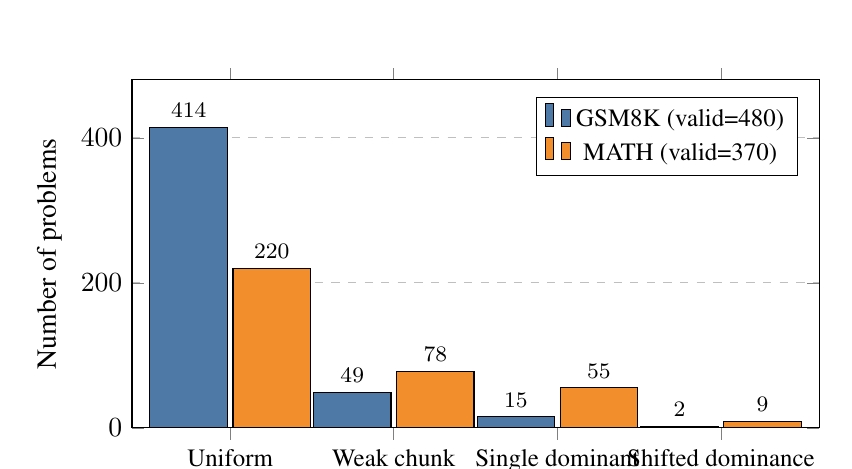
\begin{tikzpicture}
\begin{axis}[
    ybar,
    bar width=28pt,
    width=0.85\textwidth,
    height=6.0cm,
    ylabel={Number of problems},
    symbolic x coords={Uniform, Weak chunk, Single dominant, Shifted dominance},
    xtick=data,
    x tick label style={font=\small},
    ymin=0, ymax=480,
    nodes near coords,
    nodes near coords align={vertical},
    every node near coord/.append style={font=\footnotesize},
    enlarge x limits=0.2,
    legend style={at={(0.97,0.95)},anchor=north east, font=\small},
    ymajorgrids=true,
    grid style=dashed,
]
%GSM8K
\addplot[fill=cbBlue] coordinates {
    (Uniform, 414)
    (Weak chunk, 49)
    (Single dominant, 15)
    (Shifted dominance, 2)
};
% MATH
\addplot[fill=cbOrange] coordinates {
    (Uniform, 220)
    (Weak chunk, 78)
    (Single dominant, 55)
    (Shifted dominance, 9)
};
\legend{GSM8K (valid=480), MATH (valid=370)}
\end{axis}
\end{tikzpicture}
\caption{Distribution of saliency patterns across valid problems.  The majority are uniform saliency,
indicating balanced reasoning contributions across chunks.}
\label{fig:saliency-pattern-dist}
\end{figure}

The dominant pattern on GSM8K is \emph{uniform} saliency (86.3\%), indicating that
no individual chunk consistently dominates the exam outcome for most
problems.  Among these 414 uniform items, 310 (74.9\%) are
\emph{perfect uniform}. The model achieves perfect quiz and exam scores
($Q_{k,j}=1$ and $E_k=1$) on all $K=5$ runs, leaving no informative
variation to distinguish chunk contributions.
The remaining 104 uniform items show some quiz or exam variation but
still produce a balanced saliency distribution ($\hat{H} \ge 0.90$).
This high proportion of perfect uniform reflects the strong
performance of the GRPO-only model on GSM8K.

In contrast, MATH presents a substantially lower proportion of uniform
saliency (59.4\%) and a much higher fraction of weak chunk and
single dominant patterns. Among the 220 uniform items, 112 (0.51\%) are 
\emph{perfect uniform}.
This change indicates that, on harder reasoning tasks, chunk-level
contributions are more uneven and structurally sensitive, suggesting
that saliency analysis becomes more informative as task difficulty
increases.

% ────────────────────────────────────────────────────────────
\subsubsection{Quiz--Exam Predictive Relationship}
\label{sec:quiz-exam-relationship}
% ────────────────────────────────────────────────────────────

A central assumption of the proposed reward design is that intermediate
quiz performance is predictive of the correctness of the final answer.
To examine this assumption, we analyze the relationship between quiz
and exam outcomes across all individual runs on both benchmarks,
covering $480 \times 5 = 2{,}400$ runs for GSM8K and
$370 \times 5 = 1{,}850$ runs for MATH.


\paragraph{Contingency analysis.}
Table~\ref{tab:quiz-exam-contingency-gsm8k-math} presents the $2 \times 2$
contingency tables for both datasets. On GSM8K, when all quizzes pass,
the exam failure rate is only 1.63\%, but it increases to 17.44\% when
any quiz fails, a \textbf{10.7$\times$} rise. On MATH, the failure rate
increases from 10.4\% to 26.1\% (approximately \textbf{2.5$\times$}).
These results indicate that quiz failures are predictive of exam
failures on both benchmarks, although the coupling is substantially
stronger on GSM8K than on the harder MATH dataset.

\begin{table}[H]
\centering
\caption{Contingency table for quiz and exam outcomes. Quiz failure is a strong predictor of exam failure.}
\label{tab:quiz-exam-contingency-gsm8k-math}
\begin{tabular}{llccr}
\toprule
\textbf{Dataset} &  & \textbf{Exam Pass} & \textbf{Exam Fail} & \textbf{$P(\text{exam fail})$} \\
\midrule
\multirow{2}{*}{GSM8K ($n_{\text{runs}}=2{,}400$)}
& Quiz all pass & 1{,}876 &  31 & 1.63\% \\
& Quiz any fail &   407  &  86 & 17.44\% \\
\midrule
\multirow{2}{*}{MATH ($n_{\text{runs}}=1{,}850$)}
& Quiz all pass & 858 &  100 & 10.4\% \\
& Quiz any fail &   659  & 233 & 26.1\% \\
\bottomrule
\end{tabular}
\end{table}


\paragraph{Scaling effect of quiz failures.}
Beyond the binary distinction, Table~\ref{tab:dose-response-gsm8k-math} and
Figure~\ref{fig:scaling-effect-line-chart-gsm8k-math} show that the probability of exam failure 
increases monotonically with the number of quiz failures in a
single run, showing a clear upward trend.

\begin{table}[H]
\centering
\caption{Exam failure probability as a function of the number of quiz failures per run. Results are reported for GSM8K and MATH under the same $K=5$ evaluation protocol.}
\label{tab:dose-response-gsm8k-math}
\begin{tabular}{llcccc}
\toprule
\textbf{Dataset} & \textbf{\# Quiz failures} & \textbf{Exam pass} & \textbf{Exam fail}
    & \textbf{$P(\text{exam fail})$} \\
\midrule
\multirow{4}{*}{GSM8K}
& 0 & 1{,}876 &  31 &  1.63\% \\
& 1 &   341  &  41 & 10.73\% \\
& 2 &    63  &  33 & 34.38\% \\
& 3 &     3  &  12 & 80.00\% \\
\midrule
\multirow{4}{*}{MATH}
& 0 & 858 & 100 & 10.4\% \\
& 1 & 444 & 95 & 17.6\% \\
& 2 & 184 & 93 & 33.6\% \\
& 3 & 31 & 45 & 59.2\% \\
\bottomrule
\end{tabular}
\end{table}

\begin{figure}[H]
\centering
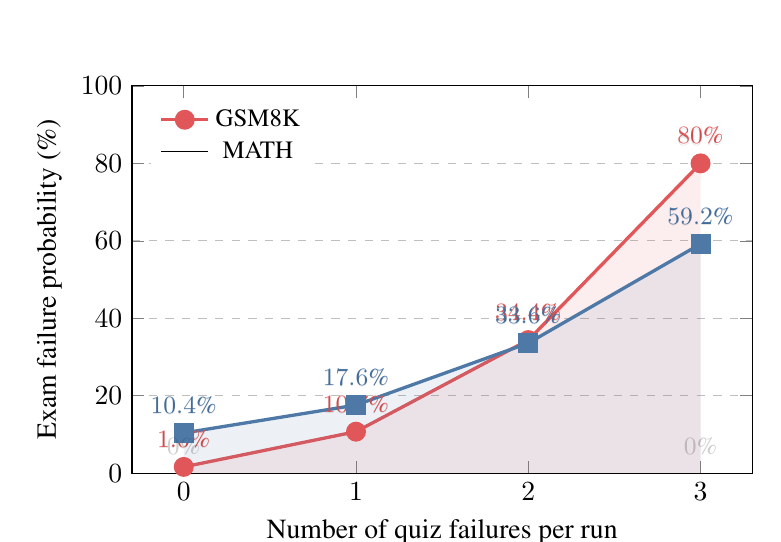
\begin{tikzpicture}
\begin{axis}[
    width=0.78\textwidth,
    height=6.5cm,
    xlabel={Number of quiz failures per run},
    ylabel={Exam failure probability (\%)},
    xtick={0,1,2,3},
    ymin=0, ymax=100,
    ytick={0, 20, 40, 60, 80, 100},
    ymajorgrids=true,
    grid style=dashed,
    mark options={solid},
    every node near coord/.append style={font=\small, above=3pt},
    nodes near coords={\pgfmathprintnumber[fixed,precision=1]{\pgfplotspointmeta}\%},
    legend style={at={(0.03,0.97)},anchor=north west, font=\small, draw=none},
]

% --- GSM8K curve ---
\addplot[
    color=cbRed,
    mark=*,
    mark size=3pt,
    line width=1.2pt,
] coordinates {
    (0, 1.63)
    (1, 10.73)
    (2, 34.38)
    (3, 80.00)
};
\addlegendentry{GSM8K}

% shade GSM8K area
\addplot[
    fill=cbRed, fill opacity=0.10, draw=none
] coordinates {
    (0, 0) (0, 1.63) (1, 10.73) (2, 34.38) (3, 80.00) (3, 0)
} \closedcycle;

% --- MATH curve ---
\addplot[
    color=cbBlue,
    mark=square*,
    mark size=3pt,
    line width=1.2pt,
] coordinates {
    (0, 10.4)
    (1, 17.6)
    (2, 33.6)
    (3, 59.2)
};
\addlegendentry{MATH}

% shade MATH area
\addplot[
    fill=cbBlue, fill opacity=0.10, draw=none
] coordinates {
    (0, 0) (0, 10.4) (1, 17.6) (2, 33.6) (3, 59.2) (3, 0)
} \closedcycle;

\end{axis}
\end{tikzpicture}
\caption{Exam failure probability increases with the number of quiz failures per run on both GSM8K and MATH. The increase is sharper on GSM8K, while MATH exhibits a higher baseline failure rate even when all quizzes pass.}
\label{fig:scaling-effect-line-chart-gsm8k-math}
\end{figure}


The growth suggests that quiz failures are not
independent. A run in which multiple intermediate steps fail is
likely to produce an incorrect final answer.
This validates the design of the quiz reward in Section~\ref{sec:quiz-reward} as a
meaningful intermediate supervision signal that quiz performance provides
dense, graded feedback that strongly correlates with final-answer
correctness.

% ────────────────────────────────────────────────────────────
\subsubsection{Positional Analysis of Quiz Failures and Weak Chunks}
\label{sec:positional-analysis}
% ────────────────────────────────────────────────────────────

We next examine \emph{where} in the reasoning trace failures are
most likely to occur.  Table~\ref{tab:quiz-fail-position-gsm8k-math} reports
quiz failure rates by chunk position across all valid runs, and
Table~\ref{tab:weak-chunk-position-gsm8k-math} reports the position distribution
of weak chunks (i.e., chunks with $w_j \le 0.10$).

\begin{table}[tbp]
\centering

\begin{minipage}[t]{0.475\textwidth}
\centering
\captionof{table}{Quiz failure rate by chunk position.}
\label{tab:quiz-fail-position-gsm8k-math}
\footnotesize
\setlength{\tabcolsep}{4pt}
\begin{tabular}{@{}llcc@{}}
\toprule
\textbf{Dataset} & \textbf{Position} & \textbf{Fail / Total} & \textbf{Fail Rate} \\
\midrule
\multirow{3}{*}{GSM8K}
& Chunk 0 (first)  & 166 / 2{,}400 & 6.92\% \\
& Chunk 1 (middle) & 213 / 2{,}400 & 8.88\% \\
& Chunk 2 (last)   & 240 / 2{,}275 & 10.55\% \\
\midrule
\multirow{3}{*}{MATH}
& Chunk 0 (first)  & 449 / 1{,}850 & 24.27\% \\
& Chunk 1 (middle) & 442 / 1{,}835 & 24.09\% \\
& Chunk 2 (last)   & 430 / 1{,}665 & 25.83\% \\
\bottomrule
\end{tabular}
\end{minipage}
\hspace{0.03\textwidth}
\begin{minipage}[t]{0.475\textwidth}
\centering
\captionof{table}{Weak chunk position distribution.}
\label{tab:weak-chunk-position-gsm8k-math}
\footnotesize
\setlength{\tabcolsep}{4pt}
\begin{tabular}{@{}llcc@{}}
\toprule
\textbf{Dataset} & \textbf{Position} & \textbf{Count} & \textbf{Proportion} \\
\midrule
\multirow{3}{*}{GSM8K}
& First  &  9 & 18.4\% \\
& Middle & 16 & 32.7\% \\
& Last   & 24 & 49.0\% \\
\midrule
\multirow{3}{*}{MATH}
& First  & 29 & 37.18\% \\
& Middle & 20 & 25.64\% \\
& Last   & 29 & 37.18\% \\
\bottomrule
\end{tabular}
\end{minipage}

\end{table}

\begin{figure}[tbp]
\centering

\begin{subfigure}[t]{0.475\textwidth}
\centering
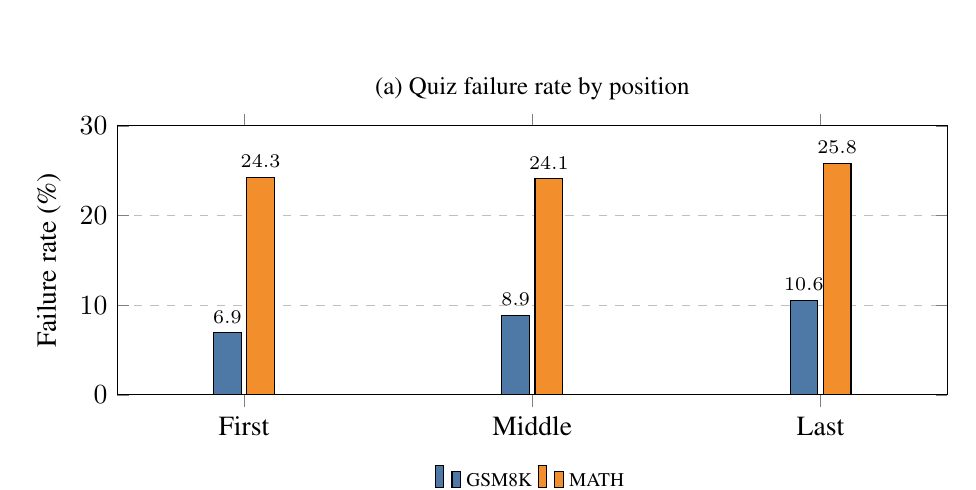
\begin{tikzpicture}
\begin{axis}[
    ybar,
    bar width=10pt,
    width=\textwidth,
    height=5.0cm,
    ylabel={Failure rate (\%)},
    symbolic x coords={First, Middle, Last},
    xtick=data,
    ymin=0, ymax=30,
    nodes near coords,
    nodes near coords align={vertical},
    every node near coord/.append style={font=\scriptsize,
        /pgf/number format/fixed, /pgf/number format/precision=1},
    enlarge x limits=0.22,
    ymajorgrids=true,
    grid style=dashed,
    title={\small (a) Quiz failure rate by position},
    legend style={at={(0.5,-0.4)},anchor=south, font=\scriptsize, draw=none, legend columns=2},
    bar shift auto,
]
% GSM8K
\addplot[fill=cbBlue] coordinates {
    (First, 6.92)
    (Middle, 8.88)
    (Last, 10.55)
};
\addlegendentry{GSM8K}

% MATH
\addplot[fill=cbOrange] coordinates {
    (First, 24.27)
    (Middle, 24.09)
    (Last, 25.83)
};
\addlegendentry{MATH}
\end{axis}
\end{tikzpicture}
\end{subfigure}
\hspace{0.03\textwidth}
\begin{subfigure}[t]{0.475\textwidth}
\centering
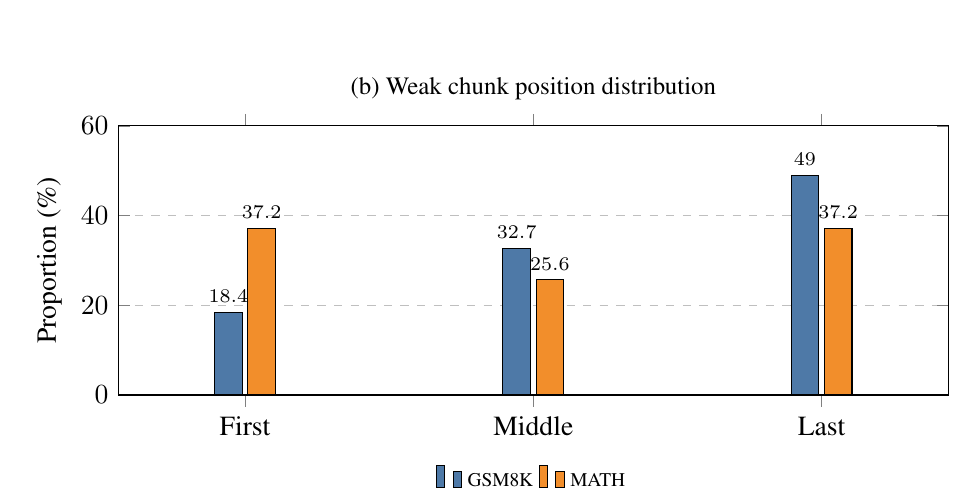
\begin{tikzpicture}
\begin{axis}[
    ybar,
    bar width=10pt,
    width=\textwidth,
    height=5.0cm,
    ylabel={Proportion (\%)},
    symbolic x coords={First, Middle, Last},
    xtick=data,
    ymin=0, ymax=60,
    nodes near coords,
    nodes near coords align={vertical},
    every node near coord/.append style={font=\scriptsize,
        /pgf/number format/fixed, /pgf/number format/precision=1},
    enlarge x limits=0.22,
    ymajorgrids=true,
    grid style=dashed,
    title={\small (b) Weak chunk position distribution},
    legend style={at={(0.5,-0.4)},anchor=south, font=\scriptsize, draw=none, legend columns=2},
    bar shift auto,
]
% GSM8K
\addplot[fill=cbBlue] coordinates {
    (First, 18.4)
    (Middle, 32.7)
    (Last, 49.0)
};
\addlegendentry{GSM8K}

% MATH
\addplot[fill=cbOrange] coordinates {
    (First, 37.18)
    (Middle, 25.64)
    (Last, 37.18)
};
\addlegendentry{MATH}
\end{axis}
\end{tikzpicture}
\end{subfigure}

\caption{Positional analysis of reasoning failures (GSM8K vs.\ MATH).
\textbf{(a)}~GSM8K shows increasing quiz failure rates toward later chunks, while MATH exhibits uniformly high failure rates across positions.
\textbf{(b)}~Weak chunks concentrate at the last position on GSM8K, whereas MATH shows a symmetric first/last distribution, suggesting distinct bottlenecks on harder problems.}
\label{fig:positional-analysis-gsm8k-math}
\end{figure}

The positional analysis reveals distinct patterns across the two
benchmarks. On GSM8K, both quiz failures and weak chunks show a clear gradient, with higher failure rates toward the final chunk. 
This pattern is consistent with error accumulation in sequential reasoning, where mistakes in earlier steps propagate and turn into failures during final integration.

In contrast, MATH does not show a monotonic positional gradient.
Quiz failure rates remain uniformly high across all positions, and weak
chunks are distributed symmetrically between the first and last
positions. This suggests that on harder problems, failures are not
confined to late chunk integration but can arise both from early problem
formulation and from final computation steps.


% ────────────────────────────────────────────────────────────
\subsubsection{Saliency Patterns}
\label{sec:qualitative-patterns}
% ────────────────────────────────────────────────────────────

To complement the aggregate statistics, we present representative
examples that illustrate the four saliency patterns identified by the
classification framework.

\begin{figure}[H]
  \centering
  \includegraphics[width=0.55\textwidth]{Image/gsm8k_94.png}
  \caption{Uniform chunk-level saliency for GSM8K-94.}
  \label{fig:saliency_uniform}
\end{figure}

\paragraph{Uniform Saliency Distributions.}
Across the GSM8K training set, we observe that the majority of examples exhibit near-uniform saliency distributions, typically close to $\{0.33, 0.33, 0.33\}$ for three reasoning chunks. 
This pattern is common in relatively short GSM8K problems, where reasoning steps are tightly coupled and errors tend to propagate uniformly to the final answer.
Uniform saliency suggests that no particular single reasoning chunk is more important or more problematic than the others. In these cases, improving performance likely requires rolling out more response samples rather than focusing on a specific intermediate step. 

\paragraph{Non-Uniform Saliency Patterns.}
In contrast to the dominant uniform case, a subset of examples exhibits non-uniform saliency distributions, where contributions differ across reasoning chunks.
Such patterns point to particular steps that have a stronger impact on the final outcome, revealing weaknesses or key operations that outcome-only supervision cannot capture.
We summarize the most common non-uniform patterns below.

\paragraph{Single Dominant Chunk.}
\begin{figure}[H]
  \centering
  \includegraphics[width=0.55\textwidth]{Image/gsm8k_162.png}
  \caption{Single dominant chunk-level saliency for GSM8K-162.}
  \label{fig:saliency_single_dominant}
\end{figure}

This distribution indicates that the final exam outcome is almost entirely determined by one intermediate segment, while the remaining chunks contribute negligibly.

Such cases typically arise when a single critical calculation determines the success. 
Once this step is correct, subsequent
reasoning has little influence on the final answer. In contrast, an
error at this step almost guaranties failure regardless of later steps.
In addition, single-dominant items show the lowest mean correct rate
(0.813) among all patterns, indicating that concentrated on a single reasoning step is associated with unreliable
performance. Among the 15 single-dominant items, 9 (60\%) have the
dominant chunk at the last position, suggesting that the final stage
computation is the critical bottleneck for these problems.

\paragraph{Weak Intermediate Chunk.}
\begin{figure}[H]
  \centering
  \begin{subfigure}{0.48\textwidth}
    \centering
    \includegraphics[width=\textwidth]{Image/gsm8k_226.png}
    \caption{GSM8K-226}
  \end{subfigure}
  \hfill
  \begin{subfigure}{0.48\textwidth}
    \centering
    \includegraphics[width=\textwidth]{Image/gsm8k_663.png}
    \caption{GSM8K-663}
  \end{subfigure}
  \caption{Weak intermediate chunks for GSM8K-226 and 663, where the middle chunk receives substantially lower saliency than the surrounding chunks.}
  \label{fig:saliency_weak_mid}
\end{figure}

In these cases, the model has difficulty with an intermediate reasoning step.
This weakness does not always lead to a wrong final answer, since later steps may sometimes compensate for earlier mistakes.
As a result, such issues are often hidden when the evaluation considers
only the final answer, even though the underlying reasoning is
unstable.  Among the 49 weak chunk items, 36 (73.5\%) have $w_j = 0.0$
(zero contribution) rather than low contribution, indicating
that the weak chunk \emph{never} successfully correlated with exam
success in any of the $K$ runs.

\paragraph{Shifted Dominance across Chunks.}
\begin{figure}[H]
  \centering
  \begin{subfigure}{0.48\textwidth}
    \centering
    \includegraphics[width=\textwidth]{Image/gsm8k_3180.png}
    \caption{GSM8K-3180-1}
  \end{subfigure}
  \hfill
  \begin{subfigure}{0.48\textwidth}
    \centering
    \includegraphics[width=\textwidth]{Image/gsm8k_3180-2.png}
    \caption{GSM8K-3180-2}
  \end{subfigure}
  \caption{Chunk-level saliency for GSM8K-3180 across different runs, showing shifted dominance in different reasoning chunk.}
  \label{fig:saliency_shifted_dominance}
\end{figure}

In this case, the responsibility for exam success alternates between
different reasoning chunks across repeated runs. Rather than revealing
one clearly weak step, shifted dominance shows that performance depends
on the combination of several reasoning segments. This pattern was
rare in our sample (only 2 items), likely because GSM8K problems
typically only have one standard solution path.

% ────────────────────────────────────────────────────────────
\subsubsection{Degenerate Saliency and Quiz--Exam Decoupling}
\label{sec:degenerate}
% ────────────────────────────────────────────────────────────

Among the 20 degenerate items (all $K=5$ exam runs incorrect), a
noteworthy subset shows \emph{decoupled} quiz and exam performance
that several degenerate
items achieved high quiz scores but consistent exam failure.
Among the 20 GSM8K degenerate items, 11 (55\%) achieved a mean quiz
score above 0.50 but failing all exam runs, and 3 items obtained
perfect quiz scores ($\bar{Q} = 1.0$) across all $K=5$ runs.

The effect is substantially more pronounced on MATH, where 130 items
are degenerate. Of these, 47 (36.2\%) maintained mean quiz scores
above 0.50, and 7 (5.4\%) achieved perfect quiz scores while
consistently failing the exam. The higher proportion of these
cases suggests that exam failure on harder problems often arises from
final-stage breakdowns or formatting issues rather than uniformly
incorrect intermediate reasoning.

Outcome only supervision treats all such cases as equally incorrect,
even when intermediate reasoning steps are largely correct and the
failure occurs only at the final integration or computation stage.

% ────────────────────────────────────────────────────────────
\subsubsection{Correct Rate and Saliency Variance}
\label{sec:correct-rate-variance}
% ────────────────────────────────────────────────────────────

To quantify the relationship between saliency structure and model
reliability, we group problems by their correct rate
($\text{correct\_rate} = n_{\text{correct}} / K$) and examine how
saliency variance changes between groups.

\begin{table}[H]
\centering
\caption{Saliency variance by correct rate group (GSM8K and MATH).
Lower correct rates correspond to higher saliency variance.}
\label{tab:correct-rate-bins-gsm8k-math}
\begin{tabular}{llcc}
\toprule
\textbf{Dataset} & \textbf{Correct Rate Group} & \textbf{Count}
    & \textbf{Mean Saliency Var} \\
\midrule
\multirow{4}{*}{\shortstack{GSM8K\\(N=500)}}
& Perfect (1.0)      & 421 & 0.010 \\
& High (0.8--0.99)   &  26 & 0.011 \\
& Medium (0.4--0.79) &  25 & 0.037 \\
& Low (0.0--0.39)    &   8 & 0.035 \\
\midrule
\multirow{4}{*}{\shortstack{MATH\\(N=500)}}
& Perfect (1.0)      & 225 & 0.038 \\
& High (0.8--0.99)   &  50 & 0.039 \\
& Medium (0.4--0.79) &  66 & 0.045 \\
& Low (0.0--0.39)    &  29 & 0.079 \\
\bottomrule
\end{tabular}
\end{table}

\begin{figure}[H]
\centering
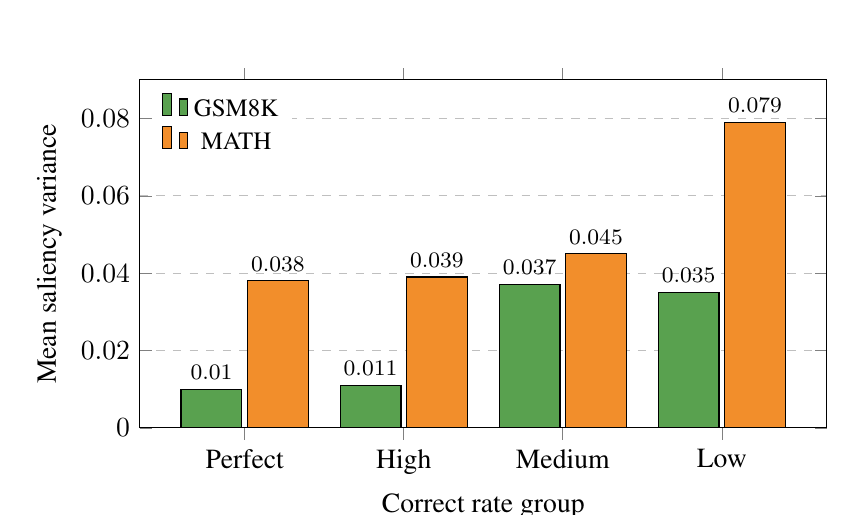
\begin{tikzpicture}
\begin{axis}[
    ybar,
    bar width=22pt,
    width=0.85\textwidth,
    height=6.0cm,
    ylabel={Mean saliency variance},
    yticklabel style={
        /pgf/number format/fixed,
        /pgf/number format/precision=3
    },
    scaled y ticks=false,
    symbolic x coords={Perfect, High, Medium, Low},
    xtick=data,
    xlabel={Correct rate group},
    ymin=0, ymax=0.09,
    nodes near coords,
    nodes near coords align={vertical},
    every node near coord/.append style={font=\footnotesize,
        /pgf/number format/fixed,
        /pgf/number format/precision=3},
    enlarge x limits=0.22,
    ymajorgrids=true,
    grid style=dashed,
    legend style={at={(0.02,0.98)},anchor=north west, font=\small, draw=none},
    bar shift auto,
]

% GSM8K
\addplot[fill=cbGreen] coordinates {
    (Perfect, 0.010)
    (High, 0.011)
    (Medium, 0.037)
    (Low, 0.035)
};
\addlegendentry{GSM8K}

% MATH
\addplot[fill=cbOrange] coordinates {
    (Perfect, 0.038)
    (High, 0.039)
    (Medium, 0.045)
    (Low, 0.079)
};
\addlegendentry{MATH}

\end{axis}
\end{tikzpicture}
\caption{Mean saliency variance by correct rate group (GSM8K and MATH).
MATH exhibits consistently higher saliency variance across all difficulty levels,
with especially large variance in the low-correct-rate regime.}
\label{fig:variance-by-correctrate-gsm8k-math}
\end{figure}

On GSM8K, problems in the medium correct-rate range (0.4--0.79)
show substantially higher saliency variance than perfectly solved
problems (0.037 vs.\ 0.010). This indicates that saliency analysis is
most informative at intermediate difficulty levels, where the model
occasionally fails and chunk-level credit assignment helps identify
which reasoning steps drive the inconsistency. For perfectly solved
problems, saliency remains largely uniform and therefore less diagnostic.

In contrast, MATH maintains relatively high saliency variance across all
difficulty groups, with especially large variance in the low-correct-rate
regime (0.079). Even perfectly solved MATH problems show higher variance than GSM8K,
indicating that structural instability persists across difficulty levels
rather than emerging only in partially solved cases.


% ────────────────────────────────────────────────────────────
\subsubsection{Summary and Implications}
\label{sec:saliency-summary}
% ────────────────────────────────────────────────────────────

The aggregate saliency analysis reveals distinct patterns across GSM8K
and MATH, with implications for reward design and targeted training.

\begin{enumerate}[nosep]

\item \textbf{Quiz rewards are predictive, but coupling strength differs.}
On GSM8K, quiz failure increases the probability of exam failure by
10.7$\times$, and the dose–response curve shows a sharp monotonic
increase (Tables~\ref{tab:quiz-exam-contingency-gsm8k-math} and
\ref{tab:dose-response-gsm8k-math}). On MATH, quiz failure remains
predictive but the effect is weaker (2.5$\times$), reflecting more
distributed sources of failure in harder reasoning tasks. Quiz rewards
therefore provide meaningful intermediate supervision on both
benchmarks with different strengths.

\item \textbf{Error localization differs across difficulty levels.}
GSM8K shows a clear late stage gradient with both quiz failures and weak
chunks concentrating in the final reasoning step
(Figure~\ref{fig:positional-analysis-gsm8k-math}). In contrast, MATH
shows uniformly high failure rates across positions and a symmetric
first/last weak-chunk distribution. This suggests that easier problems
tend to fail at integration, whereas harder problems involve multiple
structural bottlenecks.

\item \textbf{Saliency structure correlates with reliability.}
On GSM8K, single dominant problems have the lowest correct rate and
medium-difficulty problems show 3--4$\times$ higher saliency variance
(Table~\ref{tab:correct-rate-bins-gsm8k-math}), indicating that uneven
credit assignment aligns with unstable reasoning. On MATH, saliency
variance remains high across all difficulty groups, suggesting broader
structural instability rather than a narrow intermediate diagnostic
chunk.

\item \textbf{Diagnostic value depends on task regime.}
For GSM8K, saliency is most informative in the intermediate
difficulty range, where the model partially succeeds and chunk-level
variation identifies correctable weaknesses. For MATH, diagnostic
signals are present across difficulty levels, including perfectly
solved cases, suggesting that on harder tasks, improving performance may require
strengthening multiple parts of the reasoning process, rather than
focusing on a single weak chunk.

\item \textbf{Quiz--exam decoupling exposes limitations of outcome-only supervision.}
Both benchmarks contain degenerate items where quiz scores are high
but exam performance fails, with more
common on MATH. This demonstrates that outcome-only supervision cannot
distinguish globally incorrect reasoning from localized late-stage
failures, motivating chunk-aware reinforcement strategies.

\end{enumerate}

Overall, saliency analysis enables automated identification of fragile
reasoning segments without human-annotated intermediate labels. The
results suggest that targeted reinforcement should be adapted to task
difficulty. Late stage refinement is for structured, easier benchmarks,
and broader structural stabilization is for harder reasoning tasks.


\subsection{Reward Reweighting Improvements on Weak Reasoning Chunks}
\label{sec:weak_chunks}


\chapter{Conclusion and Future work}
This thesis studies how to improve mathematical reasoning in large language models under a
fully automated training pipeline. Instead of relying on human-annotated intermediate steps,
we design a quiz-augmented reward that provides denser feedback during reinforcement learning,
and we further analyze reasoning behavior using chunk-level saliency.

Overall, our results suggest that (i) reinforcement learning can significantly improve math
reasoning even without supervised fine-tuning initialization when the backbone is already
instruction-tuned, and (ii) relatively simple reward signals, if well-aligned, can be competitive
with more complex reward engineering. At the same time, our analysis also highlights several
practical limitations and open directions for future experiments.

\section{Limitations}
Although the proposed framework is fully automated and works well in our experiments, it still
has several limitations worth noting.

\paragraph{Trajectory-level credit assignment limits weak chunk repair.}
Although weak chunk reward reshaping can increase the selection pressure toward trajectories that contain fragile reasoning segments, GRPO fundamentally operates at the trajectory level with sequence-level rewards. The policy update is driven by relative ranking among complete rollouts rather than by fine-grained credit assignment within individual reasoning chunks. As a result, the method cannot directly repair a specific weak reasoning segment. Instead, it biases the probability mass toward trajectories that achieve higher overall reward. If the rollout distribution does not already contain trajectories that correct the weak segment, the algorithm has no mechanism to generate local repairs. In this sense, weak-chunk targeting under trajectory-level optimization functions as a selection bias rather than a guaranteed repair mechanism.

\paragraph{Quiz alignment is helpful but not perfect.}
The quiz mechanism improves reward density, but it depends on the quality and alignment of the
generated quizzes. Even with a filtering stage, some quizzes can still be too close to the final goal and therefore provide limited extra supervision, or slightly off-target so that learning signals that do not transfer to the original problem. This misalignment risk is
hard to remove completely without stronger verification or more expensive generation.

\paragraph{Reward design remains sensitive to task difficulty.}
Our ablation suggests quiz and step rewards help most in the ``middle'' difficulty, problems that are
not trivial, where outcome-only reward is already enough, but not so hard that the model fails too
early for intermediate feedback to matter. For challenging problems (e.g., AIME2024),
intermediate rewards are
most effective when the model can already produce partially correct reasoning states. In these cases,
further improving early-stage solution quality or using a curriculum could make the intermediate
signals more impactful.

\paragraph{SFT can reduce performance when the backbone is already instruction-tuned.}
An important empirical observation in this thesis is that applying supervised fine-tuning on synthetic
data can degrade performance relative to the original instruct model. SFT narrows the policy distribution that hurts
generalization and reduces exploration during GRPO. This effect suggests that ``more training'' is not always better when the starting model is already strong.

\paragraph{Evaluation scope and comparability.}
For GSM8K and MATH, we evaluate on a randomly sampled subset (200 problems) rather than the
full official test sets, and we use a unified prompt and answer extraction pipeline across benchmarks.
This makes the comparisons inside this thesis consistent, but it also means the absolute scores are
not directly comparable to official leaderboard numbers. In addition, since we evaluate on a sampled subset rather than the full test set, the scores can
change slightly depending on which problems are sampled. This effect is more noticeable when the
gap between methods is small.

\paragraph{Compute and engineering constraints.}
All experiments are conducted under limited hardware resources in a single-GPU setting. As a result, we use
relatively shorter generation lengths, smaller group sizes, and a narrower range of hyperparameter
search than would be feasible at larger scale. These constraints reflect a realistic development
environment, but they also reduce the extent to which we can systematically experiment stability,
sample-efficiency, and robustness across settings. In addition, chunk-level saliency analysis and
weak-chunk targeting are implemented as lightweight diagnostic. More
comprehensive variants are possible, but remain beyond the scope of this thesis.


\section{Conclusion}
This thesis proposes a practical reinforcement learning framework for improving LLM mathematical
reasoning with automated intermediate supervision. The key idea is simple that instead of asking humans
to label reasoning steps, we generate short quizzes that probe intermediate checkpoints and turn them
into reward signals. Combined with a final-answer ``exam'' reward and a lightweight step
bonus, the model receives denser feedback while still optimizing the end task.

Empirically, GRPO post-training yields substantial gains over supervised fine-tuning baselines in our
setting. A notable result is that starting directly from an instruction-tuned backbone and
applying GRPO can outperform variants that first perform SFT on MetaMathQA. This suggests that,
for modern instruct models, reinforcement learning can serve as a strong post-training mechanism by
itself, and that SFT initialization should be used carefully rather than assumed beneficial.

Beyond aggregate benchmark scores, the chunk-level saliency analysis provides a useful perspective for
understanding reasoning behavior. Many problems exhibit near-uniform saliency across chunks,
while a non-trivial subset shows dominant or weak intermediate segments. This supports the thesis
motivation that credit assignment matters in long-horizon reasoning while outcome-only signals often hide
where the reasoning actually breaks.

As a result, these findings point to a practical middle ground between expensive process
supervision and sparse outcome only optimization. We can obtain meaningful intermediate guidance
without human-labeled chains of thought, and we can do so with a pipeline that remains simple
enough to run under realistic compute constraints.

\section{Future Work}
There are several directions that would meaningfully strengthen and extend this work.

\paragraph{Chunk-level advantage and fine-grained credit assignment.}
A more fundamental extension is to move beyond trajectory-level optimization and introduce
chunk-level advantage estimation. Instead of assigning a single scalar reward to the entire rollout,
one could segment the solution into reasoning chunks and estimate advantages at the chunk level.
Policy updates would then weight token log-probabilities according to the advantage of the chunk
they belong to, enabling localized reinforcement or suppression of specific reasoning segments.
Such a mechanism would directly address the credit assignment limitation identified in this thesis,
where trajectory-level GRPO functions primarily as a selection bias over complete solutions.
Implementing chunk-level advantages would require modifications to the training loop, including
per-chunk reward modeling or value estimation, but it offers a path toward true weak reasoning repair rather than indirect selection.


\paragraph{Stronger quiz generation and verification.}
A natural next step is to improve quiz quality while keeping the pipeline automated. For example,
one could (i) generate quizzes conditioned on identified ``risky'' steps, (ii) use multiple verifiers and
agreement to reduce noise, or (iii) explicitly penalize \emph{ok\_final} quizzes so the model is not
rewarded twice for the same outcome. Another direction is to diversify quiz types (numeric
checkpoints, symbolic equivalence, unit checks) to better cover different failure modes.

\paragraph{More principled weak-chunk targeting.}
The current weak-chunk mechanism uses saliency as a diagnostic and then scales advantages to
emphasize weak segments. This could be extended in several ways: adaptive chunk sizes, curriculum
over weak patterns, or combining saliency with uncertainty signals (e.g., variance across sampled
solutions) to decide what to reinforce. Another practical improvement is to evaluate whether targeted
reinforcement improves not just accuracy but also solution stability under different decoding
temperatures.

\paragraph{Broader evaluation beyond math.}
While math is a clean domain for studying long-horizon reasoning, the same idea could apply to
other settings such as planning, tool-use, and scientific reasoning. A useful future experiment would
be to design intermediate ``quizzes'' that check subgoals or constraints (instead of intermediate
calculations) and test whether the approach generalizes.

\paragraph{Understanding when SFT helps and hurts.}
The observation that SFT can degrade performance relative to the instruct model deserves deeper
study. Future work could isolate factors such as dataset mixture, formatting constraints, and solution
style bias. One concrete direction is to compare different SFT objectives (e.g., short answer-only
vs.\ full chain-of-thought imitation) and measure how they affect RL exploration and final
generalization.

\paragraph{Scaling laws and stability.}
Finally, it would be valuable to systematically study scaling behavior: larger group sizes,
longer rollouts, and more training steps may change the trade-offs between reward complexity and
performance. A more exhaustive stability study (KL control, reward clipping, advantage
normalization variants) would also help make the approach more robust and reproducible.

\section{Final Thoughts}
This thesis started from a practical question: can we improve mathematical reasoning in LLMs
without paying the cost of human process supervision? The results suggest the answer is ``often yes,''
at least in a constrained but realistic setting. By framing intermediate supervision as automated
quizzes and combining it with reinforcement learning, we obtain a training signal that is denser than
outcome-only rewards yet far cheaper than human-labeled reasoning traces.

At a higher level, the main takeaway is not that reward engineering must be complicated, but that it
must be well-aligned. In our experiments, the strongest improvements come from a small number of
simple signals that directly reflect the task goal and the kinds of intermediate mistakes that models
make. This suggests a practical path forward: build automated feedback that resembles how humans
learn (frequent, targeted checks), keep the training objective stable, and focus on diagnosing where
reasoning fails rather than only counting final answers.

We hope these insights help future work on reinforcement learning for long-horizon reasoning tasks,
both within mathematics and beyond.

\clearpage
\phantomsection
\addcontentsline{toc}{chapter}{References}
\renewcommand{\bibname}{References}
\bibliographystyle{unsrt} 
\bibliography{references}


\appendix

% Fix weird ".1" section numbering in appendix
\renewcommand{\thesection}{A.\arabic{section}}
\titleformat{\section}{\normalfont\bfseries}{\thesection}{1em}{}
\chapter{Appendix}
\section{Prompt Template for Solution Generation}
\label{app:prompt}
\begin{lstlisting}[basicstyle=\ttfamily\small, frame=single]
You are a careful math and logic reasoning assistant.
You must first think step by step, and then give a final concise answer
that directly matches what the question is asking for.

[Instructions]
- Read the user's question carefully.
- Write your reasoning as numbered steps:
  Step 1: ...
  Step 2: ...
  Step 3: ...
  ...
- After the reasoning is complete, output ONE clear final answer.
- The final answer MUST:
  - Match the type requested in the question
    (e.g., a number, an algebraic expression, a choice like A/B/C/D/E, a probability, etc.).
  - Be as short and direct as possible (no extra explanation).
- Put the final answer on a separate line in the form:
  <final_answer>: <your answer here></final_answer>
- After you output </final_answer>, do NOT write anything else.

[Example 1 - arithmetic]
[User]
Compute 2 + 3 * 4.
[/User]

[Solution]
Step 1: According to order of operations, compute the multiplication first: 3 * 4 = 12.
Step 2: Then add 2 + 12 = 14.
<final_answer>14</final_answer>
[/Solution]

[Example 2 - multiple choice]
[User]
Two trains are moving toward each other...
(choices: A, B, C, D, E)
[/User]

[Solution]
Step 1: Convert both speeds to m/s.
Step 2: Compute the relative speed and time until they meet.
Step 3: Match the numerical result to the closest option.
<final_answer>C</final_answer>
[/Solution]

Now follow the same style for the new question.

[User]
{question}
[/User]

[Solution]
\end{lstlisting}

\section{Prompt Template for Quiz Answering}
\label{app:quiz-prompt}

\begin{lstlisting}[basicstyle=\ttfamily\small, frame=single, breaklines=true, breakatwhitespace=true]
[User Question]
{question}
[/User Question]

[Partial Solution]
{chunk text}
[/Partial Solution]

[QUIZ]
{quiz}
[/QUIZ]

[Instruction]
Only output the final answer token(s) (e.g., a number, fraction a/b, or A-E).
No words, no punctuation, no explanation.
[/Instruction]
\end{lstlisting}

\section{Prompt Template for Quiz Generation}
\label{app:quiz-generation-prompt}

\begin{lstlisting}
You are generating intermediate quizzes for math reasoning.

Given the math problem and a correct solution below, generate up to {n} quizzes.

Rules:
- Each quiz must have an answer that is ONLY one of:
  (A) a number (integer/decimal, no words),
  (B) a multiple-choice letter (A/B/C/D),
  (C) a formula in a single line using only variables/numbers and + - * / ^ ( ) (no sentences).
- Do NOT ask "what operation", "what should we do next", or any explanation-type question.
- Prefer numeric checkpoints that are critical for getting the final answer.

Return in JSON only:

{
  "quizzes": [
    {
      "question": "...",
      "answer": "..."
    }
  ]
}

Problem:
{question}

Correct solution:
{exam_answer}
\end{lstlisting}

\section{Prompt template for Quiz-Question Alignment}
\label{app:quiz-question-alignment}

\begin{lstlisting}
You judge whether quizzes align with a math word problem.
Be conservative. Do NOT solve the whole problem.
If a quiz essentially restates the original question's final goal 
(e.g., asks for the same final quantity), label it as "ok_final" even if it is grounded and useful.
\end{lstlisting}


\end{document}